%
% HSR LaTex Template
% Copyright 2012, Florian Bentele
%
% Complete LaTex template for thesis at HSR, customized
% for Prof. Dr. Peter Heinzmann
%
%
% This document is free software: you can redistribute
% it and/or modify it under the terms of the GNU
% General Public License as published by the Free
% Software Foundation, either version 3 of the License,
% or (at your option) any later version.
%
% This document is distributed in the hope that it will
% be useful, but WITHOUT ANY WARRANTY; without even the
% implied warranty of MERCHANTABILITY or FITNESS FOR A
% PARTICULAR PURPOSE. See the GNU General Public
% License for more details.
%
% You should have received a copy of the GNU General
% Public License along with this document. If not, see
% <http://www.gnu.org/licenses/>.
%

\documentclass[11pt,twoside]{hsrthesis}

%\makeindex

% do this here, so you can \gls{...} to it
%%add new glossaryentries here...

\newglossaryentry{sqlite}{
	name=SQLite,
	description={SQLite ist eine Datenbankengine, welche ohne Konfiguration auskommt. Es handelt sich dabei um eine Datenbank in einer Datei},
	first={SQLite}
}
%\makeglossaries

\begin{document}


\newcommand{\thesistitle}{Teamreview 2}
\newcommand{\thesisauthora}{Pascal Horat, Steve Gerome Kamga, Gökhan Kaya}
\newcommand{\thesisauthorb}{}
\newcommand{\thesisauthorc}{}
\newcommand{\professor}{Prof. Dr. Some Body}
\newcommand{\thesistype}{Bachelorarbeit}
\newcommand{\departement}{Abteilung Informatik}
\newcommand{\school}{Hochschule für Technik Rapperswil}
\newcommand{\term}{Frühjahrssemester 2017}
\newcommand{\thedate}{21. März 2017}
\newcommand{\timeperiode}{21.02.2012 - 01.06.2012}
\newcommand{\partner}{-}
\newcommand{\workload}{-}
\newcommand{\linktothesis}{https://moodle.hsr.ch}

\setlength{\oddsidemargin}{20mm}
\maketitle
\setlength{\oddsidemargin}{20mm}

%\chapter{Abstract}

\begin{abstract}

Vorliegendes Dokument beschreibt die Entwicklungsprozesse und das Endprodukt des TKI-Auftrags \textit{Assessment Center}.\\ In genanntem Auftrag geht es darum, ein sogenanntes Assessment zu entwickeln. Dies ist in unserem Fall ein Werkzeug, mit welchem man in der Lage sein soll, das Vorhandensein wichtiger Kompetenzen bei Elektroingenieuren zu überprüfen. Diese Kernkompetenzen müssen zuerst in Erfahrung gebracht werden. Die Idee ist es, Personalmanagementbüros und Elektroingenieure in der Industrie zum Thema zu befragen um anschliessend mittels einer Auswertung die wichtigsten Kompetenzen zu ermitteln.\\ Sobald die Kernkompetenzen bekannt sind, wird, anhand zweier selbst entwickelter Übungen, das Assessment an Probanden durchgeführt und schlussendlich ausgewertet.
\end{abstract}

\tableofcontents


% The main content
%%%%%%%%%%%%%%%%%%
\chapter{Verzeichnisse}

\section{Abbildungen}

\section{Quellen Abbildungen}
%03introduction.tex

\chapter{Ziel dieses Dokumentes}

Das Ziel dieses Dokuments ist es, die im HSR-Modul Teamkommunikation für Ingenieure erlernten Teamrollen-Modelle anwenden zu können und diese den Teammitgliedern zuzuordnen. So sollen potenzielle Stärken und Schwächen des Teams entdeckt und Konsequenzen eingeleitet werden. 

\chapter{Analyse Projektauftrag}
Die nachfolgende Analyse des Projektauftrags wurde anhand der Vorlage \textit{HSR\_Projektauftrag.docx} vorgenommen. Einige Punkte mögen daher eventuell unpassend erscheinen, wurden aber so gut wie möglich auf unser Projekt angewandt.
\section*{Assessment Center}

\section{Ausgangssituation und Kontext}
Der Stoff des Moduls Teamkommunikation für Ingenieure soll nicht nur theoretisch vermittelt, sondern auch praktisch erfahren werden können. Dazu wird ein industrienahes Projekt als Turngerät verwendet. Anhand von diesem Projekt sollen möglichst viele praktische Erfahrungen zum Thema Teamkommunikation gemacht werden. Das Turngerät ist in unserem Falle der Auftrag Assessment Center.

\subsection{Ist Situation}
Das Projekt Assessment Center soll im Dreierteam Pascal Horat, Gerome Kamga und Gökhan Kaya abgewickelt werden. Die drei Teammitglieder kannten sich im Vornherein nicht. Pascal Horat und Gökhan Kaya studieren Elektrotechnik, Gerome Kamga Maschinenbau und ist ein Austauschstudent aus Deutschland/ Kamerun.

\subsection{Problem}
Die Problemstellung besteht darin, die wichtigsten Kompetenzen von Elektroingenieuren zu ermitteln and danach ein Verfahren (= Assessment) zu entwickeln, mit dessen Hilfe das Vorhandensein der gefundenen Kernkompetenzen bei Personen geprüft werden kann.
\subsection{Rahmenbedingungen}
Für die Bearbeitung des Projekts sind die vierzehn Wochen des Frühjahrssemesters 2017 vorgesehen, wobei alle Teammitglieder vollzeitlich Vorlesungen und Praktikas besuchen. Wöchentlich findet ein vierstündiger TKI-Block (= Teamkommunikation für Ingenieure) statt. Wobei die erste Hälfte immer aus einem Theorieblock des Dozenten besteht. Somit kann gesagt werden, dass uns von der Schule aus pro Woche zwei Lektionen für die Bearbeitung des Projekts zustehen. Hier muss aber angemerkt werden, dass die Projektarbeit nicht die einzige abzugebende Arbeit für dieses Modul ist. Jeder Student hat nämlich noch drei persönliche Lernbilanzen und drei Teamreviews (werden zusammen in den Teams verfasst) abzugeben. 
\subsection{Interessensvertreter/Stakeholder}
\subsubsection{Definition}
Als Stakeholder wird eine Person oder Gruppe bezeichnet, die ein berechtigtes Interesse am Verlauf oder Ergebnis eines Prozesses oder Projektes hat \cite{wiki:Stakeholder}.

\subsubsection{Stakeholder unseres Projekts}
Da wir in unserem Projekt keine Firma als Projektpartner haben, ist neben unserem Team der einzige Stakeholder der Dozent. 
\section{Projektziele}
\subsubsection{Definition}
Projektziele sind die Aufstellung von möglichst quantifizierten Anforderungen, die erfüllt sein müssen, damit ein Projekt als erfolgreich abgeschlossen betrachtet werden kann \cite{ wiki:Projektziel}.
\subsubsection{Unsere Projektziele}
\begin{itemize}
\item Erfolgreich drei Kernkompetenzen ermitteln zu können
\item Zwei sinnvolle Übungen zu den Kernkompetenzen entwickeln
\item Die Übungen mit mindestens zwei Probanden durchzuführen, um schauen zu können ob man damit das Vorhandensein der Kernkompetenzen überprüfen kann
\item Den Projektbericht in der geforderten Qualität und Quantität zeitlich abgeben zu können
\item Möglichst viele Teamprozesse am eigenen Leib erfahren zu können
\end{itemize} 

\subsection{Systemziele}
\subsubsection{Definition}
Systemziele können erst gemessen werden, nachdem das Produkt/System für eine gewisse (definierte) Zeit im Einsatz gestanden hat. Die Verantwortung für die Erreichung der Systemziele trägt der Auftraggeber und nicht der Projektleiter.\\
Der Projektleiter muss selbstverständlich dafür besorgt sein, dass die notwendigen Ansprüche (= Anforderungen) an das Projekt erfüllt werden; d.h. dass das Produkt entsprechend ausgelegt ist \cite{page:Systemziel}.

\subsubsection{Unsere Systemziele}
Da unser Assessment nicht wirklich eine Anwendung findet, können auch keine Systemziele definiert werden. 
\subsection{Abwicklungsziele}
\subsubsection{Definition}
Die Abwicklungsziele beziehen sich auf die Projektabwicklung und bezeichnen dort grundsätzlich die Inhalte der Meilensteine (Leistung, Termine, Kosten und Qualität) bzw. welche Arbeitsergebnisse wann in welcher Form vorliegen sollen (und wie viel das kosten darf) \cite{page:Abwicklungsziel}.
\subsubsection{Unsere Abwicklungsziele}
Die definierten Meilensteine mit den entsprechenden Daten finden sich im Kapitel \ref{sec:Vorgehen} auf Seite \pageref{sec:Vorgehen}. 
\subsection{Abgrenzung}
Unser Projekt ist vollständig von den anderen Projekten und Teams im Modul abgegrenzt. Es gibt somit keine Überschneidungen. Selbstverständlich dürfen aber die andern Teams bei Fragen kontaktiert werden.
\section{Risiken und Chancen}
\subsection{Risiken}
\begin{itemize}
\item Ein Mitglied unseres Teams empfindet den Aufwand als zu hoch und meldet sich vollständig vom Modul ab
\item Die Teammitglieder finden bei der Bearbeitung des Projektes keinen gemeinsamen Nenner. Diese Möglichkeit besteht vor allem, weil sich die Mitglieder noch nicht gekannt haben im Vornherein
\item Die Zeitverhältnisse mit all den anderen Modulen sind zu knapp, es kann nicht die Zeit aufgewendet werden um eine qualitativ gute Arbeit abzuliefern
\end{itemize}
\subsection{Chancen}
\begin{itemize}
\item Die Teammitglieder empfinden das Projekt als eine positive Erfahrung und erleben Situationen, die ihnen im Berufsalltag helfen werden
\item Die eigene Erstellung eines Assessments fördert das Verständnis dafür, was von Firmen bei einem Bewerbungsverfahren verlangt wird
\end{itemize}
\subsection{Kritische Erfolgsfaktoren}
\begin{itemize}
\item Die Teammitglieder können genug Zeit in das Projekt investieren
\item Die Beziehungen innerhalb des Teams sind gut genug um eine qualitativ gute Arbeit abzuliefern
\end{itemize}

\section{Grobplanung}

\subsection{Zeitliche Abgrenzung}\label{Abgrenzung}
\begin{tabular}{ | l | l | l | l |}
    \hline
    Projektbeginn: & 20.02.2017 & Projektende: & 29.05.2017  \\ \hline
\end{tabular}

\subsection{Meilensteine}
Weitere Informationen dazu im Kapitel \ref{sec:Vorgehen} ab Seite \pageref{sec:Vorgehen}.\\

\begin{tabular}{ | p{0.3cm} | p{7.7cm} | p{4.3cm} | p{1.3cm} |}
    \hline
    \textbf{\#} & \textbf{Was?} & \textbf{Wer?} PaHo = Pascal Horat, GeKa = Gerome Kamga, GöKa = Gökhan Kaya & \textbf{Circa bis wann?} \\ \hline
    1 & Erstellen der Grobplanung in MS Project & PaHo & 12.04.17 \\ \hline
    2 & Erstellen der Struktur des Projektberichts in LaTex & GöKa & 12.04.17 \\ \hline
    3 & Fragekatalog ausarbeiten für Kernkompetenzen & GöKa, GeKa & 13.04.17 \\ \hline
    4 & Interviewpartner festlegen & PaHo, GeKa, GöKa & 21.04.17 \\ \hline
    5 & Kernkompetenzen von Ingenieuren ermitteln & PaHo, GeKa, GöKa & 28.04.17 \\ \hline
    6 & Die wichtigsten Kernkompetenzen eruieren & GeKa, GöKa & 01.05.17 \\ \hline
    7 & Zwei Übungen für Kernkompetenzen entwickeln & PaHo, GeKa, GöKa & 14.05.17 \\ \hline
    8 & Probanden organisieren & PaHo, GeKa, GöKa & 12.05.17 \\ \hline
    9 & Assessment mit Probanden durchführen & PaHo, GöKa & 19.05.17 \\ \hline
    10 & Assessment auswerten & PaHo, GöKa & 22.05.17 \\ \hline
    11 & Reflexion des Projekts & PaHo, GeKa, GöKa & 24.05.17 \\ \hline
    12 & Endüberarbeitung des Projektberichts & PaHo, GeKa, GöKa & 25.05.17 \\ \hline 
\end{tabular} 

\subsection{Diskrepanz Beginn Projekt}
Die zeitliche Diskrepanz zwischen dem Projektbeginn in Abschnitt \ref{Abgrenzung} und dem Beendigungsdatum des ersten Meilenstienes rührt daher, dass gerade am Anfang des Moduls sehr viel Zeit für die Erstellung der Teamreviews und der Lernbilanzen aufgewendet wurde.

\section{Ressourcen/Kosten}
\subsection{Personelle Ressourcen}
\begin{tabular}{| p{3cm} | p{4cm} | p{4cm} |}
\hline
\textbf{Arbeitskraft} & \textbf{Funktion} & \textbf{Stundenansatz} \\ \hline
Pascal Horat & Teamkoordinator & 45 CHF \\ \hline
Gerome Kamga & Teammitglied & 40 CHF \\ \hline
Gökhan Kaya & Teammitglied & 40 CHF \\ \hline

\end{tabular}\\

Als beratende und unterstützende Person trat der betreuende Dozent des Moduls, Dr. rer. pol Bruno Sternath, auf.

\subsection{Kosten}
\subsubsection{Personelle Kosten}
Die personellen Kosten für das ganze Projekt, wobei nur Arbeiten die direkt damit zusammenhängen miteinbezogen wurden, belaufen sich gemäss Zusammenstellung im MS Project auf 6322 CHF. Dies ergibt bei einem durchschnittlichen Stundenansatz von 41.7 CHF einen Aufwand von 50.5 Stunden Arbeit für das Projekt pro Person.

\subsubsection{Materielle Kosten}
Da aufgrund des Projekts keine materiellen Investitionen und Anschaffungen von Nöten waren, sind die Kosten in dieser Sparte marginal. Als einzige Ausgabe kann man das Ausdrucken der fertigen Arbeit zählen. Wir nehmen an, die Arbeit wird zu Überprüfungszwecken zuerst einmal komplett schwarz/weiss gedruckt um dann das fertige Produkt farbig zu Drucken. Die Kosten sind für doppelseitig schwarz/weiss zu Drucken 0.15 CHF pro Blatt und um doppelseitig farbig 0.75 CHF pro Blatt an der HSR. Bei vierzig Blättern (Vorder- und Rückseite) also etwa 80 Seiten, ergibt dies Druckkosten von 36 CHF.
\section{Projektorganisation}
Siehe im Kapitel \ref{sec:Vorgehen} ab Seite \pageref{sec:Vorgehen}.
\section{Machbarkeit}
Da schon zahlreiche andere Gruppen mit einer ähnlichen Vorbildung und Personalstärke dieses Projekt erfolgreich abschliessen konnten, wird die Machbarkeit als sehr gut eingeschätzt.

%\makeatletter				%Damit kein pagebreak bei neuem chapter
%\patchcmd{\chapter}{\if@openright\cleardoublepage\else\clearpage\fi}{}{}{} 
%Damit kein pagebreak bei neuem chapter
%\makeatother				%Damit kein pagebreak bei neuem chapter

%04chapterSelbsteinsch.tex
\chapter{Teamgrundlagen}
\label{sec:Teamgrundlagen}

\section{Teamvertrag}

Der folgende Teamvertrag wurde am Anfang des Projektes niedergeschrieben. Spätere Änderungen werden in diesem Abschnitt und im Abschnitt \ref{sec:Vorgehen} beschrieben.

\vspace{20mm}
\rule{\textwidth}{1pt}

Das Ziel dieses Dokuments ist das Festlegen allgemeiner Regeln, die für die zukünftige Teamarbeit als verbindlich gelten.\\

\begin{center}

\includegraphics[scale=0.25]{img/clock}\\
\end{center}


\begin{itemize}
\item Pünktlichkeit ist sehr wichtig. Bei mehr als 10 Minuten Verspätung, ist dies den anderen per WhatsApp zu melden
\end{itemize}

\begin{center}

\includegraphics[scale=1.1]{img/work}\\
\end{center}

\begin{itemize}
\item Falls ein Auftrag ohne akzeptable Begründung nicht erledigt wird, muss dieser auf die nächste Woche nachgeholt werden. Falls er auch dann nicht erledigt wurde, wird eine Konsequenz mit dem Dozenten erarbeitet
\end{itemize}

\begin{center}
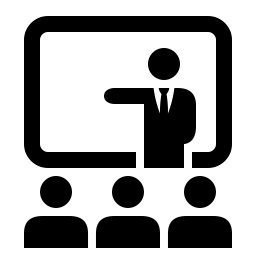
\includegraphics[scale=0.3]{img/lecture}\\
\end{center}

\begin{itemize}
\item Wenn nicht anders abgemacht, treffen wir uns jeden Montag in der Vorlesung. Falls weitere Termine notwendig sind, werden zusätzliche Sitzungen einberufen \\
\end{itemize}

\begin{center}

\includegraphics[scale=0.25]{img/communication}\\
\end{center}

\begin{itemize}
\item Als Kommunikationskanäle dienen unsere WhatsApp-Gruppe und das schulinterne E-Mail. Als Datenablage und Versionskontrolle verwenden wir GitHub. Bei grösseren Files wird die eingerichtete OneDrive-Cloud hinzugezogen\\\\
\end{itemize}

\begin{center}

\includegraphics[scale=1.2]{img/doc}\\
\end{center}

\begin{itemize}
\item Um Dokumente zu setzen, wird \LaTeX verwendet. Die nötigen Vorlagen werden, falls als sinnvoll erachtet, erstellt
\end{itemize}

\begin{center}

\includegraphics[scale=0.12]{img/boss}\\
\end{center}

\begin{itemize}
\item Da unsere Gruppenstruktur keinen eigentlichen Chef aufweist, werden folgende Verantwortungsbereiche definiert (Änderungen bei Einstimmigkeit vorbehalten):\\


\begin{itemize}
\item Projektkoordinator: Pascal Horat
\item LaTeX-Vorlagen: Pascal Horat
\item MS-Project: Steve Gerome Kamga
\item Git/Github: Gökhan Kaya  
\item Projektbericht: Pascal Horat
\item Kostenveranschlagung: Gökhan Kaya
\item Vortragsplanung: Steve Gerome Kamga
\item Teamreview: alternierend
\item Sitzungschef: alternierend
\end{itemize}
\end{itemize}


\begin{center}

\includegraphics[scale=0.3]{img/voteHand}\\
\end{center}

\begin{itemize}
\item Jede Meinungsverschiedenheit wird besprochen und falls keine Einigung erzielt werden kann, nach relativer Mehrheitswahl entschieden\\\\
\end{itemize}

\begin{center}

\includegraphics[scale=0.3]{img/performance}\\
\end{center}

\begin{itemize}
\item Unsere Teamphilosophie ist es, mit einem gegebenen Zeitaufwand ein möglichst gutes Produkt abzuliefern. Das Ziel dabei ist, möglichst viele Arbeiten während der Vorlesungszeit erledigen zu können\\\\
\end{itemize}

\begin{center}

\includegraphics[scale=0.7]{img/quality}\\
\end{center}

\begin{itemize}
\item Falls eine Person die angestrebte Qualität vernachlässigt, wird eine zweiwöchige Frist angesetzt. Hat sich in dieser Frist die Qualität der Produkte nicht verbessert, werden weitere Schritte in Absprache mit dem Dozenten eingeleitet\\\\
\end{itemize}

%\begin{tabular}{p{6.5cm}p{6.5cm}p{6.5cm}}
\begin{tabular}{p{4cm}p{5cm}p{5.5cm}}
Pascal Horat & Steve Gerome Kamga & Gökhan Kaya\\

\includegraphics[scale=0.6]{img/unterschriftPascal}&

\includegraphics[scale=0.6]{img/unterschriftGerome}&

\includegraphics[scale=0.6]{img/unterschriftGoekhan}
\end{tabular}

\section{Teamrollen}

Im Teamreview 2 wurde eine Selbsteinschätzung gemäss Belbin-Verfahren durchgeführt. Anschliessend kamen jeweils noch Fremdeinschätzungen unsererseits dazu. Der Vorgang, die Resultate und eine ausführliche Analyse mit Vergleichen sind alle im Teamreview 2 zu finden. 

\section{Teameffizienz}

Anfangs wurden alle Arbeiten im Plenum erledigt. Ein Grund dafür könnte sein, dass wir uns nicht ganz sicher waren, was genau wie zu erledigen war. So konnten wir uns ständig austauschen. Das Problem war jedoch, dass sich dieses Vorgehen als sehr ineffizient herausstellte. Der Teamvertrag musste also in einigen Punkten revidiert werden. Insbesondere wurde nun Pascal der Teamchef und verteilte die Aufträge, während wir die Aufträge so selbstständig wie möglich zu erledigen versuchten. Dies führte zu einer deutlichen Effizienzsteigerung. \\
Weiter litt die Teameffizienz deutlich daran, dass Pascal einen Monat im Militärdienst war und Gerome einige Schwierigkeiten mit der Sprache, Github und \LaTeX hatte. \\
Nichtsdestotrotz verlief die Zusammenarbeit ohne zwischenmenschliche Schwierigkeiten, was vor allem für Gökhan ein sehr wichtiger Faktor darstellte.  \\
Eine detaillierte Auseinandersetzung dazu ist im Teamreview 3 zu finden.  

%04chapterFremdeinsch.tex
\chapter{Klärung der Aufgabenstellung}

Anfangs war nicht ganz klar, wie alles von statten gehen sollte. Aus diesem Grunde haben wir uns Fragen aufgeschrieben und alle gleich in einer Sitzung mit dem Dozenten besprochen. Folgendes kam dabei raus:

\textbf{1. Was ist genau der Umfang des Assessmentberichtes?} \\
Antwort: Es wurde keine konkrete Zahl genannt. Im Umfang sind wir freigestellt.

\textbf{2. Welche Vorlage sind vorhanden?} \\
Antwort: Alles ist im Moodle vorhanden. Es wird verlangt, dass wir uns selbstständig informieren und alle Dokumente durchforsten.

\textbf{3. Muss Projektplanung mit MS Project gemacht werden? Gibt es Alternativen?}\\
Antwort: MS Project wird verlangt.

\textbf{Wird Auftrag noch spezifiziert oder müssen wir mit dem arbeiten was auf Doodle ist?} \\
Antwort: Es wird keine weitere Spezifizierungen geben.

\textbf{5. Wie muss mit allen erstellten Dokumenten verfahren werden?} \\
Antwort: Sitzungsprotokolle und Traktandenlisten usw. kommen als Anhang in den Projektbericht.


%06chapterVergleich.tex

\chapter{Vorgehen}
\label{sec:Vorgehen}

Als Pascal die ganze Koordination übernahm, erstellte er anfangs ein Grobablauf \ref{fig:grobablauf}, der uns als Grundlage und gute Übersicht dienen sollte.

\begin{figure}[ht]
	\centering
	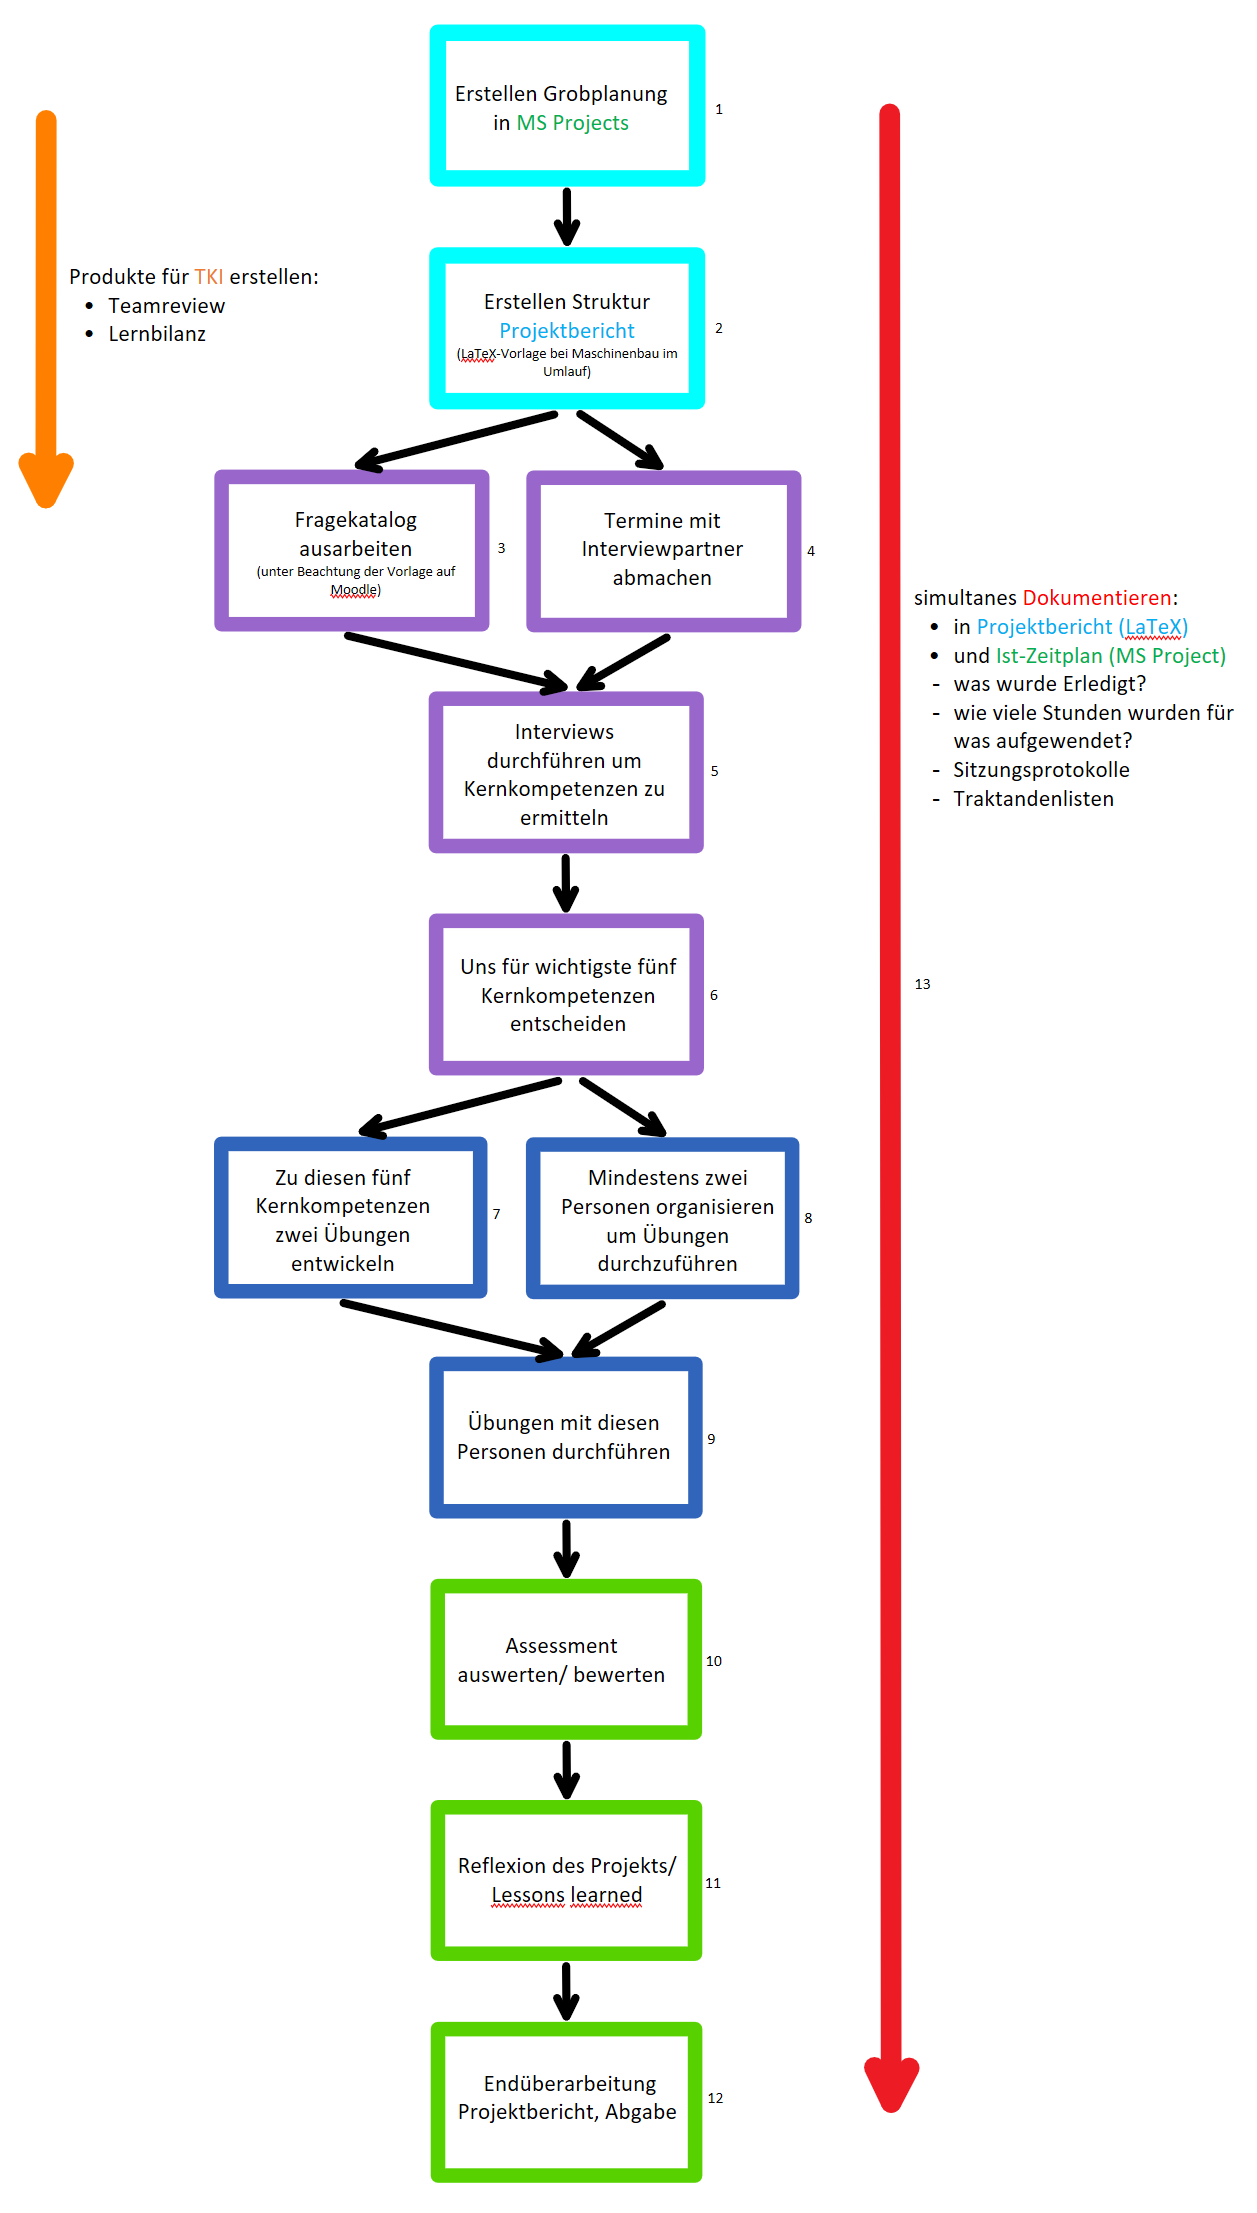
\includegraphics[width=0.9\textwidth]{images/Grobablauf.png}
	\caption{Grobablauf}
	\label{fig:grobablauf}
\end{figure}

Anschiessend hat er mittels MS Project eine Detailplanung \ref{fig:msproject} erstellt. Diese enthält alle Arbeiten inkl. Zeitvorgaben.

\begin{figure}[ht]
	\centering
	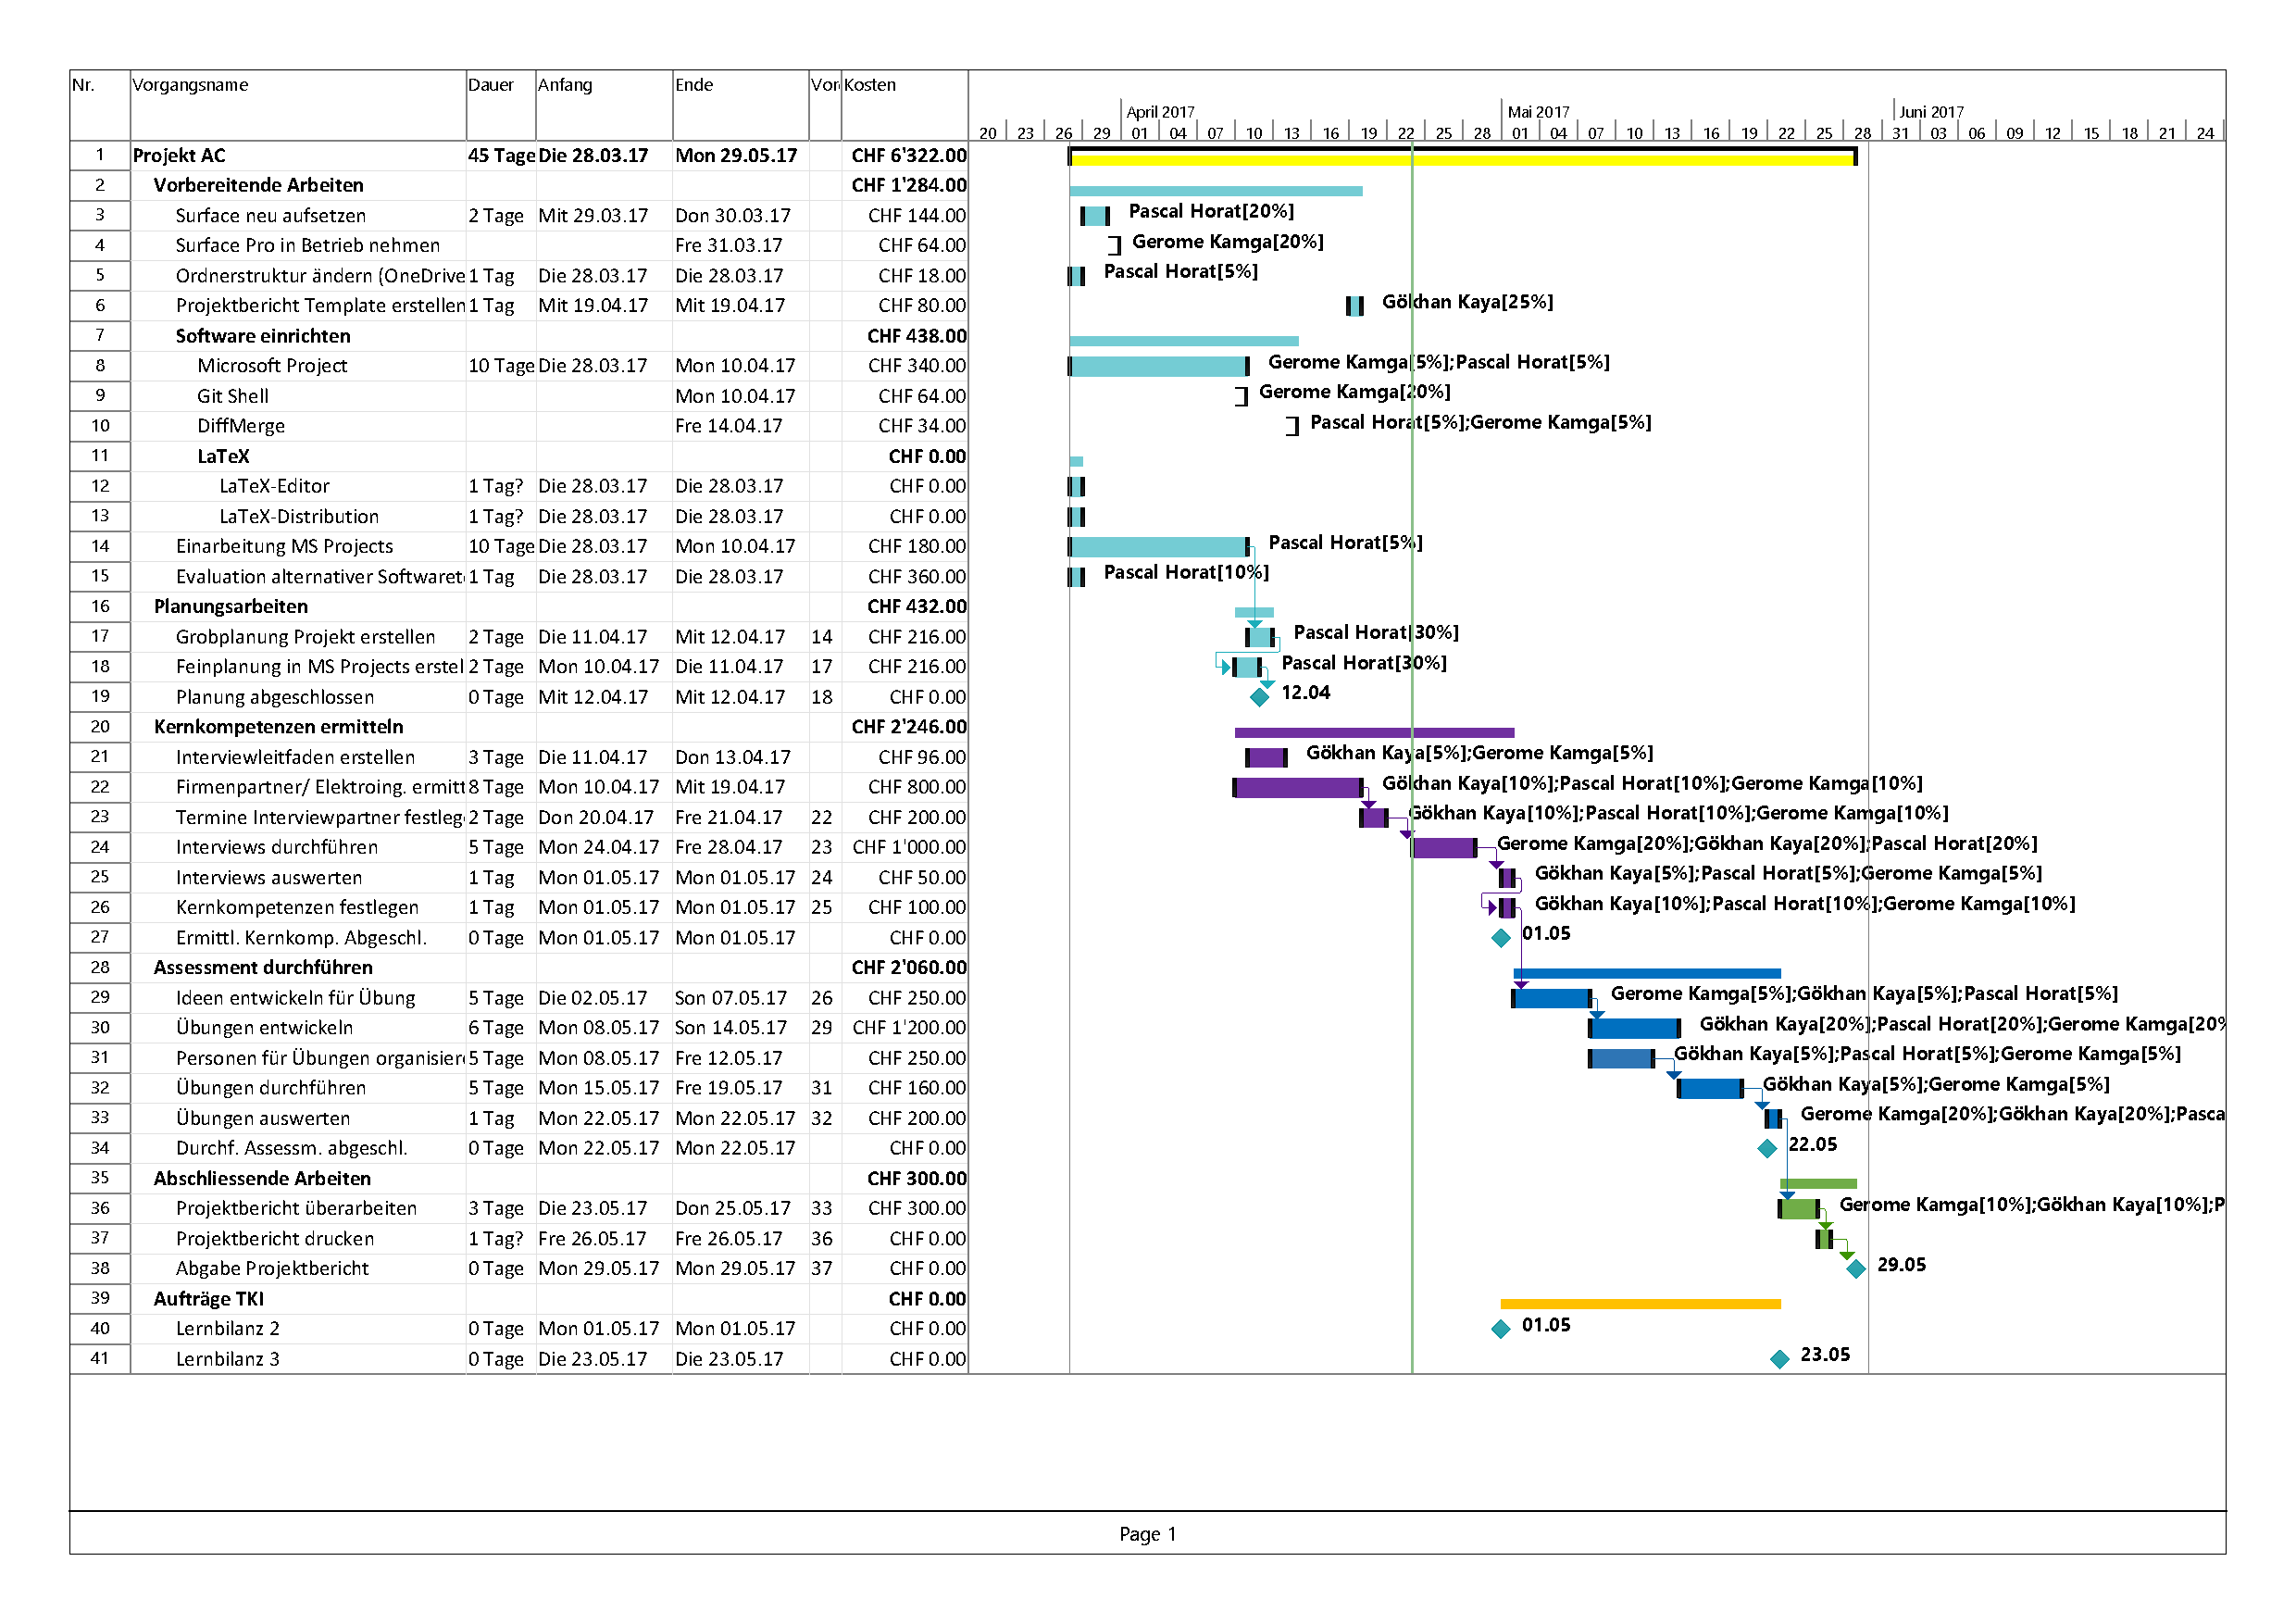
\includegraphics[width=0.9\textwidth]{images/BaselineAC2.pdf}
	\caption{Baseline in MS Project}
	\label{fig:msproject}
\end{figure}

Um die Aufträge koordinieren zu können, hat Pascal schliesslich ein Excel-File erstellt und diese auf One-Drive geladen. Dieses File liess sich von allen (jedoch nicht Gleichzeitig) online bearbeiten und abspeichern. Pascal konnte nach den Fristen seine Kommentare dazu abgeben oder falls nötig dazu auffordern einige Korrekturen vorzunehmen. Je nach Stand der Arbeit wurden die Aufträge gemäss Bild \ref{fig:auftrage} farblich markiert. Gökhan und Gerome konnten jeweils eintragen, wie viel der Aufträge (in Prozente) bereits erledigt und wieviel Zeit dafür aufgewendet wurde. 

\begin{figure}[ht]
	\centering
	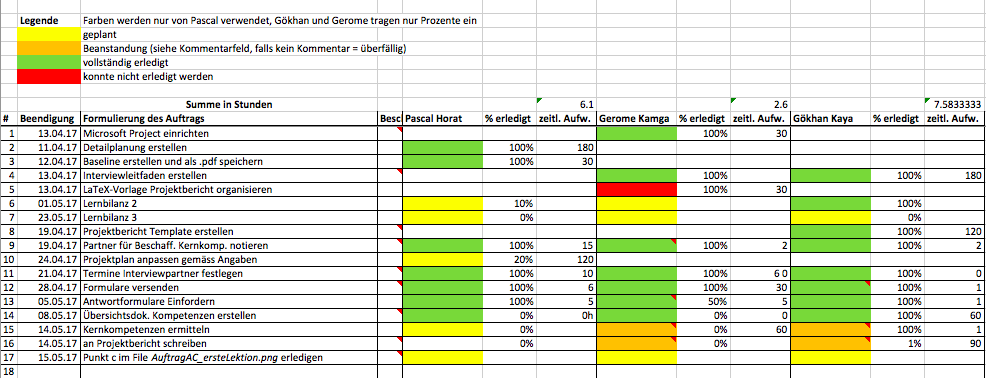
\includegraphics[width=0.5\textwidth]{images/Auftrage}
	\caption{Ausschnitt Auftragsaufteilung}
	\label{fig:auftrage}
\end{figure}

Da viele Arbeiten mittels dem Versionsverwaltungstool Git erledigt wurden, kann an dieser Stelle ebenfalls eine gute Übersicht über die tatsächlich erledigten Arbeiten gezeigt werden. Unten ist die Liste mit unseren tatsächlich hochgeladenen Änderungen inkl. unseren Kommentaren zu sehen.

%AB HIER KANN JEROME FORMATIEREN

kaya, Thu Jun 1 16:15:20 2017 +0200 : Diverse Änderungen im Abschnit Teamgrundlagen und Vorgehen \\
kaya, Thu Jun 1 15:32:12 2017 +0200 : Merge branch 'master' of https://github.com \\
kaya, Thu Jun 1 16:15:20 2017 +0200 : Diverse Änderungen im Abschnitt Teamgrundlagen und Vorgehen\\
kaya, Thu Jun 1 15:32:12 2017 +0200 : Merge branch 'master' of https://github.com/cruis1/tki merge
kaya, Thu Jun 1 15:32:03 2017 +0200 : Teil Vorgehen überarbeitet
Corumh, Thu Jun 1 15:25:52 2017 +0200 : Übung Selbstmanag. mitzut. Infos fertigg.
kaya, Thu Jun 1 14:44:34 2017 +0200 : Merge branch 'master' of https://github.com/cruis1/tki böö
kaya, Thu Jun 1 14:44:23 2017 +0200 : Teil Vorgehen geschrieben
Corumh, Thu Jun 1 14:42:44 2017 +0200 : Übung Selbstmanag. mitzut. Infos angef.
Corumh, Thu Jun 1 13:58:12 2017 +0200 : Übung Selbstmanag. verfeinert
Corumh, Thu Jun 1 13:19:40 2017 +0200 : Merge branch 'master' of https://github.com/cruis1/tki
Corumh, Wed May 31 17:51:22 2017 +0200 : Übung Selbstmanag. alle Aufgabe fertig
kaya, Wed May 31 16:02:27 2017 +0200 : Teil Klärung der Aufgabenstellung angefangen
kaya, Wed May 31 15:31:15 2017 +0200 : Merge branch 'master' of https://github.com/cruis1/tki kei ahnig was lauft
kaya, Wed May 31 15:28:27 2017 +0200 : Fragetext korrigiert
Corumh, Wed May 31 15:22:57 2017 +0200 : Merge branch 'master' of https://github.com/cruis1/tki
Corumh, Wed May 31 15:22:32 2017 +0200 : Übung Selbstmanag. E-Mail-Aufgabe fertig//
kaya, Wed May 31 15:12:52 2017 +0200 : Einleitung korrigiert
kaya, Wed May 31 14:46:12 2017 +0200 : Kapitel Teamgrundlagen geschrieben. Achtung: Kann fehler verursachen beim kompilieren
kaya, Wed May 31 12:17:54 2017 +0200 : Vorbereitungen für Teamvertrag img ordner hinzugefügt
Corumh, Wed May 31 12:16:43 2017 +0200 : Übung Selbstmanag. Kreuzwortraetsel fertig
kaya, Wed May 31 11:51:52 2017 +0200 : Erster Teil der Einleitung
Corumh, Wed May 31 11:48:57 2017 +0200 : Übung Selbstmanag. Messbericht fast fertig
kaya, Wed May 31 10:56:55 2017 +0200 : kleine korrekturen
Corumh, Wed May 31 10:49:15 2017 +0200 : Übung Selbstmanag. Messbericht weitergeschr.
kaya, Wed May 31 10:40:43 2017 +0200 : Merge branch 'master' of https://github.com/cruis1/tki testmerge
kaya, Wed May 31 10:40:15 2017 +0200 : Tabelle korrigiert
Corumh, Wed May 31 10:39:52 2017 +0200 : Übung Selbstmanag. Messbericht angef.
Kaya, Tue May 30 20:30:33 2017 +0200 : Diverse Tabellen hinzugefügt
Kaya, Tue May 30 19:56:43 2017 +0200 : Viele Korrekturen und weitere Arbeiten
kaya, Tue May 30 18:11:52 2017 +0200 : Teil Test1 hinzugefügt
Corumh, Tue May 30 16:27:24 2017 +0200 : Übung Selbstmanag. Bewertungskriterien weiter beschr.
Corumh, Tue May 30 15:19:04 2017 +0200 : Beobachtungsinstr. Selbstmanag. Bewertungskriterien beschr.
kaya, Tue May 30 14:47:56 2017 +0200 : nüt
Corumh, Tue May 30 14:29:34 2017 +0200 : Beobachtungsinstr. Selbstmanag. Bewertung
Corumh, Tue May 30 13:53:05 2017 +0200 : Beobachtungsinstr. Selbstmanag. Aufgaben weiter beschrieben
Corumh, Mon May 29 17:14:46 2017 +0200 : Beobachtungsinstr. Selbstmanag. Aufgaben beschrieben
Corumh, Mon May 29 16:10:04 2017 +0200 : Beobachtungsinstr. Selbstmanag. Detail beschrieben
Corumh, Mon May 29 16:06:30 2017 +0200 : Beobachtungsinstr. Selbstmanag. weiter beschrieben
Corumh, Mon May 29 15:56:12 2017 +0200 : Beobachtungsinstr. Selbstmanag. beschrieben
Kaya, Thu May 25 20:42:47 2017 +0200 : Korrekturen und weitere Arbeiten
Corumh, Sun May 14 16:07:20 2017 +0200 : Projektbericht Fehler behoben
kaya, Mon May 8 16:01:52 2017 +0200 : readme update
kaya, Mon May 8 16:00:37 2017 +0200 : readme update
kaya, Mon May 8 15:52:42 2017 +0200 : korrekturen
kaya, Mon May 8 15:40:18 2017 +0200 : Kernkompetenz Auswertung hinzugefügt, Assessmentbericht Interviewteil weitergeschrieben
kaya, Mon May 8 14:59:29 2017 +0200 : HILFE file überarbeitet
kaya, Mon May 8 14:58:12 2017 +0200 : HILFE file erstellt für die hartnäckige merge konflikt
Corumh, Mon Apr 24 16:35:48 2017 +0200 : Projektbericht Referenz Website
kaya, Mon Apr 24 16:31:32 2017 +0200 : ksjdksj
Corumh, Mon Apr 24 16:26:53 2017 +0200 : Projektbericht Referenz Website
Corumh, Mon Apr 24 16:26:05 2017 +0200 : Projektbericht Referenz Website
kaya, Mon Apr 24 16:21:51 2017 +0200 : nüt spannends
kaya, Mon Apr 24 15:11:00 2017 +0200 : Ordner Projektbericht gelöscht
kaya, Mon Apr 24 12:12:08 2017 +0200 : Fragekatalog verbessert 2
kaya, Mon Apr 24 12:05:55 2017 +0200 : Fragenkatalog korrigiert
kaya, Wed Apr 19 19:09:19 2017 +0200 : Assessmentbericht template fertig
kaya, Wed Apr 19 15:34:54 2017 +0200 : Fragekatalog nachgebessert
kaya, Wed Apr 12 21:02:19 2017 +0200 : Fragenkatalog angepasst
Corumh, Mon Apr 3 23:26:16 2017 +0200 : TR3 Orthografie korrigiert
Corumh, Mon Apr 3 23:02:35 2017 +0200 : TR3 komplett überarbeitet
Corumh, Mon Apr 3 20:29:41 2017 +0200 : TR3 Protokoll eingefügt
kaya, Mon Apr 3 20:00:33 2017 +0200 : TR3 fast fertig
kaya, Mon Apr 3 18:45:59 2017 +0200 : Gruppeneinschätzung fertig
kaya, Mon Apr 3 16:48:33 2017 +0200 : TR3 continue
Corumh, Mon Apr 3 16:01:09 2017 +0200 : TR3 Web-Pic eingefügt
Corumh, Mon Apr 3 15:57:15 2017 +0200 : Merge branch 'master' of https://github.com/cruis1/tki
kaya, Mon Apr 3 15:56:59 2017 +0200 : Arbeit...
Corumh, Mon Apr 3 14:52:12 2017 +0200 : TR2 Änderig
Corumh, Mon Apr 3 14:08:39 2017 +0200 : TR3 Vorlage pagebreak entfernt
kaya, Mon Apr 3 14:04:13 2017 +0200 : TR3 vorlage angepasst
Corumh, Mon Apr 3 02:27:49 2017 +0200 : TR3 Vorlage Fehler entfernt
kaya, Mon Mar 27 16:41:16 2017 +0200 : nichts nennenswertes
Corumh, Mon Mar 27 15:50:50 2017 +0200 : TR3 Vorlage angefangen
Corumh, Mon Mar 27 12:11:55 2017 +0200 : TR2 in finale Form gebracht
kaya, Mon Mar 27 11:08:49 2017 +0200 : pagebreak aenderungen auskommentiert
Corumh, Mon Mar 27 01:59:09 2017 +0200 : TR2 zusätzliche Literatur eingefügt
Corumh, Mon Mar 27 00:38:32 2017 +0200 : TR2 kompl. überarb. (Rechtschreibef.) und erweitert
Corumh, Sun Mar 26 17:45:31 2017 +0200 : TR2 fast fertig
Corumh, Sun Mar 26 15:27:03 2017 +0200 : an TR2 weitergearbeitet
SteveGerome, Sun Mar 26 15:16:44 2017 +0200 : weitergeschrieben TR2
Corumh, Sun Mar 26 14:55:44 2017 +0200 : an TR2 weitergearbeitet, Bilder eingefügt
Corumh, Thu Mar 23 14:24:16 2017 +0100 : an TR2 weitergearbeitet, Bilder eingefügt
Corumh, Thu Mar 23 14:03:00 2017 +0100 : .rtf gelöscht
Corumh, Thu Mar 23 13:59:07 2017 +0100 : .log gelöscht
Corumh, Thu Mar 23 13:57:40 2017 +0100 : TR2 Formattierung verschönert und weitergeschrieben
Corumh, Thu Mar 23 13:16:42 2017 +0100 : TR2 weitergearbeitet
SteveGerome, Wed Mar 22 21:23:31 2017 +0100 : zweiter Commit :-)
Corumh, Wed Mar 22 21:18:40 2017 +0100 : einige Korrekturen in TR2
SteveGerome, Wed Mar 22 21:15:22 2017 +0100 : erster Commit :-)
Corumh, Wed Mar 22 20:27:56 2017 +0100 : neueste Teamreview 2 Version Upload
kaya, Wed Mar 22 20:22:35 2017 +0100 : shit happened
kaya, Wed Mar 22 20:15:19 2017 +0100 : Selbsteinschätzung bearbeitet
Corumh, Wed Mar 22 20:10:43 2017 +0100 : hoffentlich klappts
kaya, Wed Mar 22 20:06:50 2017 +0100 : Merge branch 'master' of https://github.com/cruis1/tki
kaya, Wed Mar 22 20:06:26 2017 +0100 : Selbsteinschätzung überarbeitet
Corumh, Wed Mar 22 20:05:09 2017 +0100 : hoffentlich klappts
kaya, Wed Mar 22 19:45:55 2017 +0100 : Merge branch 'master' of https://github.com/cruis1/tki
kaya, Wed Mar 22 19:44:30 2017 +0100 : Fremdeinschätzung grob ferig
Corumh, Wed Mar 22 19:34:07 2017 +0100 : zum Abgliche
Corumh, Wed Mar 22 19:02:33 2017 +0100 : resolve merge error
Corumh, Wed Mar 22 18:45:58 2017 +0100 : Teamreview 2 Selbsteinsch. bearb
kaya, Wed Mar 22 18:45:31 2017 +0100 : test
kaya, Wed Mar 22 18:38:25 2017 +0100 : Merge branch 'master' of https://github.com/cruis1/tki
kaya, Wed Mar 22 18:34:32 2017 +0100 : removed Fremdeinschätzung
Corumh, Wed Mar 22 18:32:15 2017 +0100 : Teamreview 2 Selbsteinsch. bearb
kaya, Wed Mar 22 18:23:28 2017 +0100 : selbsteinschätzung erstellt
kaya, Wed Mar 22 17:04:09 2017 +0100 : selbsteinschätzung erstellt
Corumh, Tue Mar 21 17:35:53 2017 +0100 : Teamreview 2 weitererstellt, Referenzen funktionieren
Corumh, Tue Mar 21 17:32:52 2017 +0100 : Teamreview 2 weitererstellt, Referenzen funktionieren
Corumh, Tue Mar 21 13:56:24 2017 +0100 : Teamreview 2 Struktur erstellt, Referenzen funktionieren
Corumh, Tue Mar 21 12:09:38 2017 +0100 : Teamreview 2 Template angefangen
Corumh, Tue Mar 21 11:30:41 2017 +0100 : Ordnerstruktur geändert und noch mehr aufgeräumt
Corumh, Tue Mar 21 11:18:35 2017 +0100 : Ordnerstruktur geändert und aufgeräumt
Corumh, Tue Mar 21 11:10:12 2017 +0100 : Upload TR2
Corumh, Mon Mar 20 20:12:37 2017 +0100 : Penis
Corumh, Mon Mar 20 19:28:05 2017 +0100 : Upload TR2
Corumh, Mon Mar 20 16:13:56 2017 +0100 : Upload TR2
Corumh, Mon Mar 20 15:07:02 2017 +0100 : Upload TR2
Corumh, Mon Mar 20 13:58:25 2017 +0100 : Upload Vorlage TR2
Corumh, Mon Mar 20 12:29:35 2017 +0100 : Reflexion Sitzung finalisiert
Corumh, Fri Mar 17 17:07:49 2017 +0100 : Reflexion Sitzung erstellt
Corumh, Fri Mar 17 16:22:08 2017 +0100 : Traktl. final.
Corumh, Thu Mar 16 20:41:02 2017 +0100 : Upload Traktl. akt.
Corumh, Thu Mar 16 20:10:54 2017 +0100 : Upload Traktl.
Corumh, Thu Mar 16 19:40:46 2017 +0100 : Konflikt bereinige
Corumh, Mon Mar 13 20:53:49 2017 +0100 : Reflexion TR1 erstellt
kaya, Mon Mar 13 17:19:59 2017 +0100 : Merge branch 'master' of https://github.com/cruis1/tki
kaya, Mon Mar 13 17:06:10 2017 +0100 : Name angepasst
kaya, Mon Mar 13 17:04:04 2017 +0100 : Name angepasst
kaya, Mon Mar 13 17:02:42 2017 +0100 : Name angepasst
Corumh, Mon Mar 13 16:46:47 2017 +0100 : Reflexion TR1 erstellt
kaya, Mon Mar 13 16:32:36 2017 +0100 : Änderungen an trakdandenliste
kaya, Mon Mar 13 16:13:56 2017 +0100 : Trakdandenliste explizit vervollständigt
kaya, Mon Mar 13 15:42:03 2017 +0100 : Fragenkatalog fertiggestellt
kaya, Mon Mar 13 15:10:35 2017 +0100 : Fragenkatalog Vorlage erstellt
kaya, Mon Mar 13 14:31:25 2017 +0100 : Fragenkatalog erstellt
Corumh, Mon Mar 13 12:35:32 2017 +0100 : Merge branch 'master' of https://github.com/cruis1/tki
Corumh, Mon Mar 13 12:34:18 2017 +0100 : Regeldokument finalisiert
Columh, Sun Mar 12 23:49:13 2017 +0100 : Add files via upload
kaya, Sun Mar 12 20:20:00 2017 +0100 : trakdandenliste\_ vorlage grob fertig
kaya, Sun Mar 12 18:50:06 2017 +0100 : trakdandenliste erstellt
Corumh, Thu Mar 9 17:49:18 2017 +0100 : Regeldokument erweitert mit Bildern
Corumh, Thu Mar 9 10:47:33 2017 +0100 : Regeldokument erweitert
Corumh, Tue Mar 7 13:54:55 2017 +0100 : Regeldokument erstellt
kaya, Mon Mar 6 16:56:25 2017 +0100 : Aufträge aktualisiert
kaya, Mon Mar 6 16:29:39 2017 +0100 : teamreview update
kaya, Mon Mar 6 15:29:30 2017 +0100 : teamreview bearbeitet
kaya, Mon Mar 6 14:55:55 2017 +0100 : Ordner umbenannt und teamreview erstellt
Corumh, Mon Mar 6 14:07:14 2017 +0100 : LaTex Template verbessert
Corumh, Mon Mar 6 14:01:18 2017 +0100 : LaTex Template erstellt
Corumh, Mon Mar 6 12:02:56 2017 +0100 : LaTex Template angefangen
Corumh, Sun Mar 5 20:23:42 2017 +0100 : ToDo angepasst
cruis1, Sun Mar 5 00:18:42 2017 +0100 : Delete\_ config.yml
kaya, Sun Mar 5 00:14:02 2017 +0100 : Merge branch 'master' of https://github.com/cruis1/tki
cruis1, Sun Mar 5 00:10:44 2017 +0100 : Delete\_ config.yml
kaya, Sun Mar 5 00:04:13 2017 +0100 : doodle zu moodle geändert :)
cruis1, Sun Mar 5 00:01:11 2017 +0100 : Set theme jekyll-theme-cayman
kaya, Sat Mar 4 23:52:00 2017 +0100 : Alle files synchronisiert md file update
kaya, Sat Mar 4 23:36:00 2017 +0100 : Links hinzugefügt
cruis1, Sat Mar 4 23:31:16 2017 +0100 : Delete new.md
kaya, Sat Mar 4 23:09:51 2017 +0100 : edit readme and add new.md
cruis1, Sat Mar 4 22:15:50 2017 +0100 : Initial commit

%BIS HIER

%BEFEHL: git log --pretty=format:"%an, %ar : %s"
%BEFEHL evt. besser: git log --pretty=format:"%an, %ad : %s"
%https://git-scm.com/book/tr/v2/Git-Basics-Viewing-the-Commit-History

%07chapterZusammenfasssung.tex

\chapter{Interview}

\section{Teamideen}

\section{Interviewleitfaden}

Die Interviewleitfragen wurden mithilfe der Website \cite{Schluesselqualifikationen} erstellt. Daraus wurden zehn Schlüsselkompetenzen ausgewählt und eine Umfrage erstellt, womit die Wichtigkeit der einzelnen Schlüsselkompetenzen im Alltag eines Junior Elektroingenieur ermittelt werden sollten. Die Fragen konnten jeweils mit \textbf{sehr wichtig}, \textbf{ziemlich wichtig} und \textbf{nicht wichtig} markiert werden.   

%\footnote{Text}

\section{Interviewpartner Auswahl}

Die erstellten Umfragen haben wir anschliessend jeweils zwei bis drei uns bekannten Elektroingenieuren zugeschickt. Von den acht zugeschickten Formularen, haben wir fünf ausgefüllt zurückbekommen.
Die ausgefüllten Formulare sind im Anhang \ref{sec:Anhang} beigefügt. 

\section{Auswertung der Interviews}

Die Auswertung der Formulare erfolgte mittels einer einfachen Excel Tabelle \ref{fig:tabkernkomp}. Um herauszufinden welche Schlüsselkompetenzen wichtig waren, wurden pro Schlüsselkompetenz Punkte verteilt. Dabei entsprach ''sehr Wichtig'' plus einem Punkt, ''ziemlich wichtig'' null Punkten und ''nicht Wichtig'' minus einem Punkt. Die Summe der Punkte ist im Bild \ref{fig:auswerkomp} dargestellt. 

\begin{figure}[ht]
	\centering
	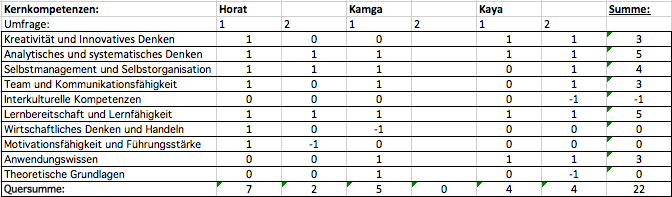
\includegraphics[width=1.1\textwidth]{images/Tabelle_Kernkompetenzen.png}
	\caption{Tabelle Kernkompetenzen}
	\label{fig:tabkernkomp}
\end{figure}

\begin{figure}[ht]
	\centering
	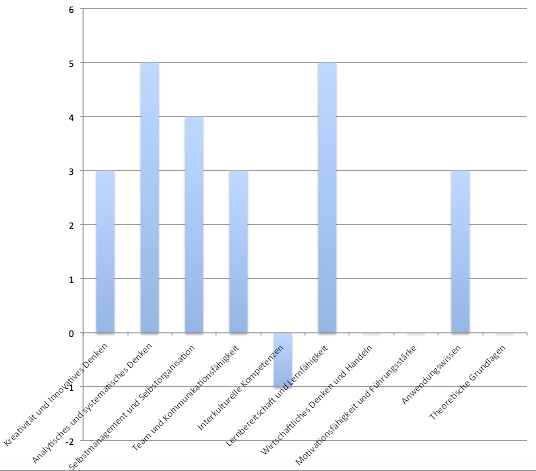
\includegraphics[width=0.9\textwidth]{images/Auswertung_kernkompetenzen.png}
	\caption{Auswertung Kernkompetenzen}
	\label{fig:auswerkomp}
\end{figure}


Interessant sind unter anderem, dass Interkulturelle Kompetenzen als die unwichtigste Kompetenz bewertet wurde. Auch schienen die befragten die theoretischen Grundlagen als kaum relevant einzuschätzen.


%08chapterKonsequenzen.tex
\chapter{Assessment}

\section{Auswahl der wichtigsten Kernkompetenzen}

Gemäss Bild \ref{fig:auswerkomp} haben sich folgende drei Kernkompetenzen als die Wichtigsten herausgestellt:

\begin{enumerate} 
\item{Logisches und analytisches Denken}
\item{Lernbereitschaft und Lernfähigkeit}
\item{Selbstmanagement und Selbstorganisation}
\end{enumerate}

\section{Übung 1: Logisches und analytisches Denken, Lernbereitschaft und Lernfähigkeit}

\section{Übung 2: Selbstmanagement und Selbstorganisation}

Mit Hilfe von dieser Übung soll ersichtlich werden, wie ausgeprägt die Kernkompetenz der Selbstorganisation beim Bewerber ist. Auch werden hier Elemente von Fachwissen und Lernbereitschaft angeschnitten. Anhand vordefinierter Kriterien soll es den Personen, welche das Assessment durchführen, möglich sein, eine valide und objektive Bewertung vornehmen zu können.

\subsection{Idee/ Grobbeschreibung}

Der Bewerber erhält vier bis fünf verschiedene, einfach scheinende Aufgaben welche er zu erledigen hat. Dies kann zum Beispiel das Ausrechnen von Schaltungsparametern einer Operationsverstärker-Schaltung, das Berechnen einer
mathematischen Aufgabe, das typografische korrigieren eines Messberichtes, das Antworten auf eine E-Mail, das Berechnen einer Emitterschaltung und so weiter sein. Die verschiedenen Aufgaben müssen zu unterschiedlichen Zeiten abgegeben werden, zusätzlich haben sie unterschiedliche Prioritäten. Die Abgabezeiten werden am Anfang mündlich bekannt gegeben. Der Bewerber hat Papier und Stift zur Verfügung.
Beim Erledigen der Aufgaben bemerkt er, dass die Reihenfolge der Aufgaben eine Rolle spielt, denn gewisse Aufgaben hängen von anderen ab. Die ganze Aufgabenstellung muss so ausgearbeitet sein, dass er nur mit
guter Planung (Zeitplanung / Prioritätenplanung), die Aufgaben zufriedenstellend erledigen kann.

Als Überschneidung mit der Lernbereitschaftsübung wird dem Bewerber zuallererst das Eisenhower-Prinzip erklärt, um dann direkt in oben beschriebener Übung zu schauen ob er es Anwenden kann, also bereit war, es zu Erlernen. 

Auf was von Assessmentseite geachtet wird:
\begin{itemize}
\item Macht er sich bei der Erläuterung der Aufgaben Notizen?
\item Schafft er sich eine Übersicht über die zu Erledigenden Arbeiten oder arbeitet er wild drauflos?
\item Erstellt er eine Zeitplanung?
\item Kategorisiert er die Aufgaben nach Dringlichkeit und Wichtigkeit (Eisenhower)?
\item Notiert er sich Fragen um Unklarheiten zu beseitigen (ihm muss vorher kommuniziert werden, das Fragen stellen erlaubt ist)?
\item Informiert er die Personen welche das Assessment durchführen wenn er es nicht schafft einen Auftrag innerhalb der Zeitfrist zu erledigen?
\end{itemize}

Mit dieser Übung wird eine Situation simuliert, welche in der Arbeitswelt so eins zu eins auftreten kann. Nämlich, verschiedene Aufgaben mit unterschiedlicher Priorität in einem begrenzten Zeitfenster erfolgreich bewältigen zu können.

\subsection{Detailbeschreibung}

An die vom Bewerber zu erledigenden Aufgaben werden folgende Kriterien gestellt:

\begin{itemize}
\item Sie soll einen Bezug zu Arbeiten haben, welche im Alltag eines Elektroingenieurs auftreten
\item Der Schwierigkeitsgrad soll so gewählt werden, dass sich der Bewerber nicht in der Aufgabe verlieren kann \item Es soll nur wenig Fachwissen zum Lösen der Aufgabe nötig sein, da das Überprüfen ebendieser nicht das Ziel ist
\item Es muss die Möglichkeit bestehen, die Aufgabe von anderen abhängig zu machen
\end{itemize}

Um testen zu können, ob der Bewerber sich zuerst ein Bild über alle zu erledigenden Aufgaben macht, muss jede Aufgabe von einer anderen abhängig sein, so dass es schlussendlich nur eine logische Abfolge gibt. Schafft er sich nämlich am Anfang keine Übersicht, sondern beginnt wahllos, so muss er rückwirkend Änderungen an vorhergehenden Aufgaben vornehmen, was ihn Zeit kostet.

Die einzig richtige Abfolge der Aufgaben ist folgende:

\subsubsection{Aufgabe 1: Korrektur Messbericht}
Dem Bewerber wird ein unvollständiger Messbericht mit typographischen Fehlern ausgehändigt, welche er korrigieren soll. % \ref{sec:Anhang}
Dies ist die erste Aufgabe, da die Resultate der Messung im Bericht Auswirkungen auf die Auslegung der Operationsverstärkerschaltung haben.

\subsubsection{Aufgabe 2: Berechnung Operationsverstärkerschaltung}
Das Resultat dieser Aufgabe ist eine vollständig berechnete Operationsverstärkerschaltung. Die Art der Schaltung wie auch die Werte der Bauelemente muss der Bewerber selber erarbeiten. Eine Notiz im Messbericht (vorherige Aufgabe) weist ihn darauf hin, ein Bauteil anders einzusetzen. Ignoriert er diese Notiz, muss er die ganze Berechnung wiederholen.

\subsubsection{Aufgabe 3: Beantwortung formelles E-Mail}
Ein Vorgesetzter braucht einige Angaben unseres Bewerbers, eine davon sind die Werte der Operationsverstärkerschaltung. Diese Aufgabe ist somit von der Vorhergehenden abhängig. Im E-Mail beschreibt der Vorgesetzte auch gleich noch den Typ des Transistors für die Emitterschaltung.

\subsubsection{Aufgabe 4: Berechnung Emitterschaltung}
Eine Emitterstufe soll berechnet werden. Diese sollte der Einfachheit halber die gleiche Ausgangsimpedanz wie die Operationsverstärkerschaltung aufweisen, ist somit also von Aufgabe 2 und drei abhängig. 

\subsubsection{Aufgabe ohne Reihenfolge: Kreuzworträtsel}
Der Teamleiter löst für sein Leben gerne Kreuzworträtsel in der Mittagspause. Da er ein sehr gründlicher Mensch ist, ist es ihm ein Bedürfnis, das Kreuzworträtsel vollständig zu haben. Leider kennt er nicht alle Antworten. Weil er aber weiss, dass der Bewerber ein ausgeprägtes Allgemeinwissen hat, gibt er ihm den Auftrag dieses während der Arbeitszeit zu vervollständigen. Diese Aufgabe hat die geringste Priorität, sie ist von keiner anderen Aufgabe abhängig und von ihr sind keine anderen Aufgaben abhängig.

\subsection{Bewertung}

Um eine objektive Bewertung vornehmen zu können, müssen die Bewertungskriterien und ihre Gewichtung im Vornherein klar definiert sein.

Die oben erwähnten Kriterien werden erweitert und mit folgender Gewichtung versehen:


\subsubsection{Macht der Bewerber sich Notizen?}
Der Ablauf der Übung wird dem Bewerber nur mündlich mitgeteilt. Ihm werden Stift und Papier bereitgestellt. Die mitgeteilten Informationen beinhalten auch die Prioritäten und Abgabezeiten der verschiedenen Aufgaben. Wenn der Bewerber sich keine Notizen macht, wird er sich wahrscheinlich nicht alles merken können. 

bei diesem Punkt wird darauf geachtet ob und in welchem Masse der Bewerber Notizen nimmt.

\begin{center}
  \begin{tabular}{ | p{4cm} | p{1cm} |}
   \hline
   \textbf{Ausprägung} & \textbf{Punkte} \\ \hline
   macht keine Notizen & 0 \\ \hline
   macht wenige Notizen & 1 \\ \hline
   macht viele Notizen & 2 \\ \hline
   notiert sich alles  & 3\\ \hline
  \end{tabular}
\end{center}


\subsubsection{Schafft er sich eine Übersicht über die Arbeiten?}

\begin{center}
  \begin{tabular}{ | p{4cm} | p{1cm} |}
   \hline
   \textbf{Ausprägung} & \textbf{Punkte} \\ \hline
   macht keine Notizen & 0 \\ \hline
   macht wenige Notizen & 1 \\ \hline
   macht viele Notizen & 2 \\ \hline
   notiert sich alles  & 3\\ \hline
  \end{tabular}
\end{center}


\begin{itemize}
\item Macht er sich bei der Erläuterung der Aufgaben Notizen?
\item Erstellt er eine Zeitplanung?
\item Kategorisiert er die Aufgaben nach Dringlichkeit und Wichtigkeit (Eisenhower)?
\item Notiert er sich Fragen um Unklarheiten zu beseitigen (ihm muss vorher kommuniziert werden, das Fragen stellen erlaubt ist)?
\item Informiert er die Personen welche das Assessment durchführen wenn er es nicht schafft einen Auftrag innerhalb der Zeitfrist zu erledigen?
\end{itemize}


\section{Ausarbeitung}

\section{Ablauf des Assessments}

\section{Aufgabenstellung}
\chapter{Bewertung Probanden}
\section{Einleitung}
Um die Tauglichkeit unserer ausgedachten Übungen, wie auch deren Schwierigkeitsgrad einschätzen zu können, wurde das Verhalten der Bewerber während dem  Assessment von uns beobachtet und mit den im Kapitel \ref{Assessment} auf Seite \pageref{Assessment} beschriebenen Bewertungskriterien eingeschätzt.\\
Die Bewertung wird unten, nach den geprüften Personen sortiert, aufgeführt.

\section{Tomo Bogdanovic}
\subsection{Übung 1: Analytisches und systematisches Denken, Lernbereitschaft und Lernfähigkeit}
\subsubsection{Resultate der Bewertungskriterien}

\subsubsection{Verschafft er sich zuerst einen Überblick?}
\begin{tabular}{| l | c | c | c |}
  \hline	
  \textbf{Ausprägung} & \textbf{Punkte lb \& lf} & \textbf{Punkte lg \& an} & \textbf{Punkte sm \& so} \\
  \hline  		
  Schafft sich keinen Überblick & 0 & 0 & 0 \\ 
  \hline
  Schafft sich fast keinen Überblick & 1 & 0 & 1 \\ 
  \hline
  Schafft sich Überblick & \circletext{2} & \circletext{0} & \circletext{2} \\
  \hline  
  Verschafft sich sehr genauen Überblick & 3 & 0 &  3 \\
  \hline  
\end{tabular}

\subsubsection{Ist eine Methodik zu erkennen oder wird ziellos gesucht?}
\begin{tabular}{| l | c | c | c |}
  \hline	
  \textbf{Ausprägung} & \textbf{Punkte lb \& lf} & \textbf{Punkte lg \& an} & \textbf{Punkte sm \& so} \\
  \hline  		
  Gar keine Methodik & 0  & 0 & 0 \\ 
  \hline
  Nur wenig Methodik & 1 & 0 & 1 \\ 
  \hline
  Gute Methodik & \circletext{2} & \circletext{0} & \circletext{2} \\
  \hline  
  Sehr strukturierte Vorgehensweise & 3 & 0 &  3 \\
  \hline  
\end{tabular}

\subsubsection{Wie sicher fühlt sich die Person während der Präsentation?}
\begin{tabular}{| l | c | c | c |}
  \hline	
  \textbf{Ausprägung} & \textbf{Punkte lb \& lf} & \textbf{Punkte lg \& an} & \textbf{Punkte sm \& so} \\
  \hline  		
  Sehr unsicher & 0  & 0 & 0 \\ 
  \hline
  Eher unsicher & 0 & 0 & 0 \\ 
  \hline
  Eher sicher & \circletext{0} & \circletext{1} & \circletext{1} \\
  \hline  
  Sehr selbstsicher & 0 & 2 &  2 \\
  \hline  
\end{tabular}


\subsubsection{Wie genau/verständlich konnte der Prozess erklärt werden. Wurden die wichtigsten Punkte erwähnt?}
\begin{tabular}{| l | c | c | c |}
  \hline	
  \textbf{Ausprägung} & \textbf{Punkte lb \& lf} & \textbf{Punkte lg \& an} & \textbf{Punkte sm \& so} \\
  \hline  		
  Hat Prozess nicht verstanden & 0 & 0 & 0 \\ 
  \hline
  Hat Prozess etwas verstanden & 1 & 1 & 1 \\ 
  \hline
  Hat Prozess gut verstranden & \circletext{2} & \circletext{2} & \circletext{2} \\
  \hline  
  Hat Prozess hervorragend verstanden & 3 & 3 &  3 \\
  \hline  
\end{tabular}

\subsubsection{Wurden Fremdwörter verwendet oder alles in eigene Worte übersetzt?}
\begin{tabular}{| l | c | c | c |}
  \hline	
  \textbf{Ausprägung} & \textbf{Punkte lb \& lf} & \textbf{Punkte lg \& an} & \textbf{Punkte sm \& so} \\
  \hline  		
  Keine Fremdwörter verwendet & 0 & 0 & 0 \\ 
  \hline
  Wenig Fremdwörter verwendet & 1 & 0 & 0 \\ 
  \hline
  Einige Fremdwörter verwendet & \circletext{2} & \circletext{0} & \circletext{0} \\
  \hline  
  Sehe viele Fremdwörter verwendet & 3 & 0 &  0 \\
  \hline  
\end{tabular}

\subsubsection{Wurde visuell gearbeitet? (Damit sind die Notizen inbegriffen)}
\begin{tabular}{| l | c | c | c |}
  \hline	
  \textbf{Ausprägung} & \textbf{Punkte lb \& lf} & \textbf{Punkte lg \& an} & \textbf{Punkte sm \& so} \\
  \hline  		
  Keine & 0  & 0 & 0 \\ 
  \hline
  Kaum & 1 & 1 & 1 \\ 
  \hline
  Einige & \circletext{2} & \circletext{2} & \circletext{2} \\
  \hline  
  Sehe viele & 3 & 3 & 3 \\
  \hline  
\end{tabular}

\subsubsection{Wurden die Erklärungen strukturiert?}
\begin{tabular}{| l | c | c | c |}
  \hline	
  \textbf{Ausprägung} & \textbf{Punkte lb \& lf} & \textbf{Punkte lg \& an} & \textbf{Punkte sm \& so} \\
  \hline  		
  Gar nich & 0 & 0 & 0 \\ 
  \hline
  Kaum & 1 & 1 & 1 \\ 
  \hline
  Genügend & 2 & 2 & 2 \\
  \hline  
  Sehr gute Struktur & \circletext{3} & \circletext{3} & \circletext{3} \\
  \hline  
\end{tabular}

\subsubsection{Wie viel wurde über den Prozess gesprochen? Wurde unnötig über Nebensächlichkeiten geredet?}
\begin{tabular}{| l | c | c | c |}
  \hline	
  \textbf{Ausprägung} & \textbf{Punkte lb \& lf} & \textbf{Punkte lg \& an} & \textbf{Punkte sm \& so} \\
  \hline  		
  Viele Nebensächlichkeiten & 0  & 0 & 0 \\ 
  \hline
  Einige Nebensächlichkeiten & 1 & 1 & 1 \\ 
  \hline
  Kaum Nebensächlichkeiten & 2 & 2 & 2 \\
  \hline  
  Keine Nebensächlichkeiten & \circletext{3} & \circletext{3} & \circletext{3} \\
  \hline  
\end{tabular}

\subsubsection{Wirkte die Person interessiert?}
\begin{tabular}{| l | c | c | c |}
  \hline	
  \textbf{Ausprägung} & \textbf{Punkte lb \& lf} & \textbf{Punkte lg \& an} & \textbf{Punkte sm \& so} \\
  \hline  		
  Gar nicht & 0  & 0 & 0 \\ 
  \hline
  Etwas & 1 & 0 & 0 \\ 
  \hline
  Interessiert & 2 & 0 & 0 \\
  \hline  
  Sehr Interessiert & \circletext{3} & \circletext{0} & \circletext{0} \\
  \hline  
\end{tabular}


\subsubsection{Summe der erreichten Punkte}
\begin{center}
  \begin{tabular}{ | p{7cm} | p{3cm} | p{3cm} |}
   \hline
   \textbf{Kernkompetenz} & \textbf{erreichte Punkte} & \textbf{maximale Punkte} \\ \hline
   Analytisches und systematisches Denken & 11 & 14\\ \hline
  Lernbereitschaft und Lernfähigkeit & 19 & 24\\ \hline
   Selbstmanagement und Selbstorganisation & 15 & 20\\ \hline
   \textbf{Total Übung 1} & \textbf{45} & \textbf{58}\\ \hline
  \end{tabular}
\end{center}

\subsubsection{Vorgehen des Kandidaten}
Anfangs schaute sich Tomo den Wikipedia Artikel an und las die Einleitung und den Theorieteil durch.  Anschliessend suchte er im Internet einfachere Erklärungen. Nach 5 Minuten einlesen begann er sich erst seine Notizen zu machen. Gegen den Schluss suchte er noch Bilder vom Prozess selbst und las noch etwas zum der Geschichte der Polymerase Kettenreaktion.

\subsubsection{Anmerkungen/Präsentation}
Tomo hatte vorher kein Vorwissen. Er meinte, dass er sich an eine Animation erinnern kann, wo DNA repliziert wird. Ich gehe davon aus, dass die DNA-Polymerase während der Replikation der DNA gezeigt wurde. Trotz des Videos konnte er nicht mit Sicherheit sagen, wie die DNA-Repliziert wird. Seine Vermutung war anfangs, dass die Primer aneinander gehängt werden und so den ganzen Strang replizieren. Er kam erst mit Nachfragen darauf, dass dies wahrscheinlich nicht der Fall sein wird. \\
Sonst wurde der Prozess gut erklärt. Die Präsentation war gut strukturiert und er behalf sich mit visuellen Darstellungen.

\subsection{Übung 2: Selbstmanagement und Selbstorganisation}
\subsubsection{Resultate der Bewertungskriterien}
\begin{center}
  \begin{tabular}{ | p{9cm} | p{1cm} |}
   \hline
   \textbf{macht sich der Proband Notizen?} & \textbf{Punkte} \\ \hline
   macht keine Notizen & 0 \\ \hline
   macht wenige Notizen & 1 \\ \hline
   macht viele Notizen & \circletext{2} \\ \hline
   notiert sich alles  & 3\\ \hline
   \textbf{schafft sich der Proband Übersicht?} & \textbf{Punkte} \\ \hline
   schafft sich keine Übersicht & 0 \\ \hline
   schafft sich fast keine Übersicht & 1 \\ \hline
   schafft sich Übersicht & \circletext{2} \\ \hline
   studiert die Aufgabenstellungen gründlich  & 3\\ \hline
   \textbf{erstellt der Proband eine Zeitplanung?} & \textbf{Punkte} \\ \hline
   erstellt keine Zeitplanung & 0 \\ \hline
   erstellt so etwas wie eine Zeitplanung & \circletext{1} \\ \hline
   erstellt eine gute Zeitplanung & 2 \\ \hline
   erstellt detail. Zeitplanung inkl. Reservezeiten  & 3\\ \hline
   \textbf{wendet der Proband das Eisenhower-Prinzip an?} & \textbf{Punkte} \\ \hline
   wendet Eisenhower-Prinzip nicht an & 0 \\ \hline
   versucht das Eisenhower-Prinzip anzuwenden & \circletext{1} \\ \hline
   wendet Eisenhower-Prinzip richtig an & 2 \\ \hline
   wendet Eisenhower-Prinzip korrekt an und leitet dadurch Konsequenzen für die Bearbeitung der Aufgaben ab  & 3\\ \hline
   \textbf{notiert sich der Proband Fragen?} & \textbf{Punkte} \\ \hline
   notiert keine Fragen & \circletext{0} \\ \hline
   notiert sich wenige relevante Fragen & 1 \\ \hline
   notiert einige relevante Fragen & 2 \\ \hline
   notiert und stellt alle relevanten Fragen  & 3\\ \hline
   \textbf{informiert der Proband über seinen Arbeitsstand?} & \textbf{Punkte} \\ \hline
   informiert den Prüfer nicht über den Arbeitsstand & \circletext{0} \\ \hline
   gibt fast keine Informationen weiter & 1 \\ \hline
   gibt viele Informationen an den Prüfer weiter & 2 \\ \hline
   gibt alle relevanten Informationen zeitgerecht an den Prüfer weiter & 3\\ \hline
  \end{tabular}
\end{center}
\begin{center}
  \begin{tabular}{ | p{11cm} | p{1cm} |}
   \hline
   \textbf{Ausprägung analytisches Denken} & \textbf{Punkte} \\ \hline
   es fällt dem Geprüften sehr schwer die Aufgabenstellungen zu verstehen & 0 \\ \hline
   der Geprüfte bei einigen Aufgabenstellungen Mühe sie zu verstehen  & 1 \\ \hline
   der Geprüfte hat wenig Mühe die Aufgabenstellungen zu verstehen & \circletext{2} \\ \hline
   dem Geprüften waren alle Aufgabenstellungen sofort klar & 3\\ \hline
   \textbf{Ausprägung systematisches Denken} & \textbf{Punkte} \\ \hline
   der Geprüfte hat grosse Mühe, die Verknüpfungen zwischen den Aufgaben zu verstehen & 0 \\ \hline
    der Geprüfte hat teilweise Mühe, die Verknüpfungen zwischen den Aufgaben zu verstehen & 1 \\ \hline
   der Geprüfte findet und versteht die Abhängigkeiten der Aufgaben & \circletext{2} \\ \hline
   findet und versteht die Abhängigkeiten der Aufgaben auf Anhieb & 3\\ \hline
  \end{tabular}
\end{center}

\subsubsection{Summe der erreichten Punkte}

\begin{center}
  \begin{tabular}{ | p{7cm} | p{3cm} | p{3cm} |}
   \hline
   \textbf{Kernkompetenz} & \textbf{erreichte Punkte} & \textbf{maximale Punkte} \\ \hline
   Selbstmanagement und Selbstorganisation & 6 & 18\\ \hline
   Analytisches und systematisches Denken & 4 & 6\\ \hline
   \textbf{Total Übung 2} & \textbf{10} & \textbf{24}\\ \hline
  \end{tabular}
\end{center}

\subsubsection{Anmerkungen}
Obwohl dem Probanden deutlich mitgeteilt wurde, dass Fragen erlaubt sind und auch einige Unklarheiten herrschten, vergass er, fragen zu stellen. Als ich ihm im Feedback-Gespräch mitteilte, dass die Aufgaben gar nicht ohne Nachfragen beim Prüfer zu lösen seien, zeigte er sich beschämt, dass er keine Fragen gestellt hatte.



\section{Michel André Nyffenegger}
\subsection{Übung 1: Analytisches und systematisches Denken, Lernbereitschaft und Lernfähigkeit}
\subsubsection{Resultate der Bewertungskriterien}

\subsubsection{Verschafft er sich zuerst einen Überblick?}
\begin{tabular}{| l | c | c | c |}
  \hline	
  \textbf{Ausprägung} & \textbf{Punkte lb \& lf} & \textbf{Punkte lg \& an} & \textbf{Punkte sm \& so} \\
  \hline  		
  Schafft sich keinen Überblick & \circletext{0} & \circletext{0} & \circletext{0} \\ 
  \hline
  Schafft sich fast keinen Überblick & 1 & 0 & 1 \\ 
  \hline
  Schafft sich Überblick & 2 & 0 & 2 \\
  \hline  
  Verschafft sich sehr genauen Überblick & 3 & 0 &  3 \\
  \hline  
\end{tabular}

\subsubsection{Ist eine Methodik zu erkennen oder wird ziellos gesucht?}
\begin{tabular}{| l | c | c | c |}
  \hline	
  \textbf{Ausprägung} & \textbf{Punkte lb \& lf} & \textbf{Punkte lg \& an} & \textbf{Punkte sm \& so} \\
  \hline  		
  Gar keine Methodik & 0 & 0 & 0 \\ 
  \hline
  Nur wenig Methodik & \circletext{1} & \circletext{0} & \circletext{1} \\ 
  \hline
  Gute Methodik & 2 & 0 & 2 \\
  \hline  
  Sehr strukturierte Vorgehensweise & 3 & 0 &  3 \\
  \hline  
\end{tabular}

\subsubsection{Wie sicher fühlt sich die Person während der Präsentation?}
\begin{tabular}{| l | c | c | c |}
  \hline	
  \textbf{Ausprägung} & \textbf{Punkte lb \& lf} & \textbf{Punkte lg \& an} & \textbf{Punkte sm \& so} \\
  \hline  		
  Sehr unsicher & 0  & 0 & 0 \\ 
  \hline
  Eher unsicher & 0 & 0 & 0 \\ 
  \hline
  Eher sicher & \circletext{0} & \circletext{1} & \circletext{1} \\
  \hline  
  Sehr selbstsicher & 0 & 2 &  2 \\
  \hline  
\end{tabular}

\subsubsection{Wie genau/verständlich konnte der Prozess erklärt werden. Wurden die wichtigsten Punkte erwähnt?}
\begin{tabular}{| l | c | c | c |}
  \hline	
  \textbf{Ausprägung} & \textbf{Punkte lb \& lf} & \textbf{Punkte lg \& an} & \textbf{Punkte sm \& so} \\
  \hline  		
  Hat Prozess nicht verstanden & \circletext{0} & \circletext{0} & \circletext{0} \\ 
  \hline
  Hat Prozess etwas verstanden & 1 & 1 & 1 \\ 
  \hline
  Hat Prozess gut verstranden & 2 & 2 & 2 \\
  \hline  
  Hat Prozess hervorragend verstanden & 3 & 3 &  3 \\
  \hline  
\end{tabular}

\subsubsection{Wurden Fremdwörter verwendet oder alles in eigene Worte übersetzt?}
\begin{tabular}{| l | c | c | c |}
  \hline	
  \textbf{Ausprägung} & \textbf{Punkte lb \& lf} & \textbf{Punkte lg \& an} & \textbf{Punkte sm \& so} \\
  \hline  		
  Keine Fremdwörter verwendet & 0  & 0 & 0 \\ 
  \hline
  Wenig Fremdwörter verwendet & 1 & 0 & 0 \\ 
  \hline
  Einige Fremdwörter verwendet & 2 & 0 & 0 \\
  \hline  
  Sehe viele Fremdwörter verwendet & \circletext{3} & \circletext{0} &  \circletext{0} \\
  \hline  
\end{tabular}

\subsubsection{Wurde visuell gearbeitet? (Damit sind die Notizen inbegriffen)}
\begin{tabular}{| l | c | c | c |}
  \hline	
  \textbf{Ausprägung} & \textbf{Punkte lb \& lf} & \textbf{Punkte lg \& an} & \textbf{Punkte sm \& so} \\
  \hline  		
  Keine & 0  & 0 & 0 \\ 
  \hline
  Kaum & 1 & 1 & 1 \\ 
  \hline
  Einige & 2 & 2 & 2 \\
  \hline  
  Sehe viele & \circletext{3} & \circletext{3} & \circletext{3} \\
  \hline  
\end{tabular}

\subsubsection{Wurden die Erklärungen strukturiert?}
\begin{tabular}{| l | c | c | c |}
  \hline	
  \textbf{Ausprägung} & \textbf{Punkte lb \& lf} & \textbf{Punkte lg \& an} & \textbf{Punkte sm \& so} \\
  \hline  		
  Gar nich & 0  & 0 & 0 \\ 
  \hline
  Kaum & 1 & 1 & 1 \\ 
  \hline
  Genügend & 2 & 2 & 2 \\
  \hline  
  Sehr gute Struktur & \circletext{3} & \circletext{3} & \circletext{3} \\
  \hline  
\end{tabular}

\subsubsection{Wie viel wurde über den Prozess gesprochen? Wurde unnötig über Nebensächlichkeiten geredet?}
\begin{tabular}{| l | c | c | c |}
  \hline	
  \textbf{Ausprägung} & \textbf{Punkte lb \& lf} & \textbf{Punkte lg \& an} & \textbf{Punkte sm \& so} \\
  \hline  		
  Viele Nebensächlichkeiten & \circletext{0} & \circletext{0} & \circletext{0} \\ 
  \hline
  Einige Nebensächlichkeiten & 1 & 1 & 1 \\ 
  \hline
  Kaum Nebensächlichkeiten & 2 & 2 & 2 \\
  \hline  
  Keine Nebensächlichkeiten & 3 & 3 & 3 \\
  \hline  
\end{tabular}

\subsubsection{Wirkte die Person interessiert?}
\begin{tabular}{| l | c | c | c |}
  \hline	
  \textbf{Ausprägung} & \textbf{Punkte lb \& lf} & \textbf{Punkte lg \& an} & \textbf{Punkte sm \& so} \\
  \hline  		
  Gar nicht & 0 & 0 & 0 \\ 
  \hline
  Etwas & 1 & 0 & 0 \\ 
  \hline
  Interessiert & \circletext{2} & \circletext{0} & \circletext{0} \\
  \hline  
  Sehr Interessiert & 3 & 0 & 0 \\
  \hline  
\end{tabular}


\subsubsection{Summe der erreichten Punkte}
\begin{center}
  \begin{tabular}{ | p{7cm} | p{3cm} | p{3cm} |}
   \hline
   \textbf{Kernkompetenz} & \textbf{erreichte Punkte} & \textbf{maximale Punkte} \\ \hline
   Analytisches und systematisches Denken & 7 & 14\\ \hline
  Lernbereitschaft und Lernfähigkeit & 12 & 24\\ \hline
   Selbstmanagement und Selbstorganisation & 8 & 20\\ \hline
   \textbf{Total Übung 1} & \textbf{27} & \textbf{58}\\ \hline
  \end{tabular}
\end{center}

\subsubsection{Vorgehen des Kandidaten}
Michel ging anfangs, wie alle anderen Testkandidaten, dazu über den Wikipedia Artikel zu lesen. Gleich am Anfang begann er damit sich ein Mindmap zu zu zeichnen. Er las dann die Einleitung des Wikipedia Artikels und schliesslich denn den Praxis-Teil. Damit verbrachte er die ersten 6 Minuten und Scrollte auch nicht weiter nach unten um zu sehen, was noch wichtigeres stehen könnte. Somit sah er den Teil, wo der Theoretische Ablauf erklärt wurde, erst nach 6 Minuten. Als er diesen Teil dann auch gelesen hatte, scrollte er schlussendlich alles durch. Die Zeit war dann bereits abgelaufen und das Resultat war dann auch wie erwartet. Der Einstieg der Präsentation war zwar sehr gelungen und er konnte eine gutes Mindmap vorweisen und die technischen Begriffe erwähnen, jedoch wusste er nicht, was diese Bedeuten und den Prozess hatte er nicht ansatzweise verstanden. 

\subsubsection{Präsenation}

Der Einstieg der Präsentation war zwar sehr gelungen, auch konnte er eine gutes Mindmap vorweisen und die technischen Begriffe erwähnen, jedoch wusste er nicht, was diese bedeuten und den Prozess hatte er nicht ansatzweise verstanden. 

\subsection{Übung 2: Selbstmanagement und Selbstorganisation}
\subsubsection{Resultate der Bewertungskriterien}
\begin{center}
  \begin{tabular}{ | p{9cm} | p{1cm} |}
   \hline
   \textbf{macht sich der Proband Notizen?} & \textbf{Punkte} \\ \hline
   macht keine Notizen & 0 \\ \hline
   macht wenige Notizen & \circletext{1} \\ \hline
   macht viele Notizen & 2 \\ \hline
   notiert sich alles  & 3\\ \hline
   \textbf{schafft sich der Proband Übersicht?} & \textbf{Punkte} \\ \hline
   schafft sich keine Übersicht & 0 \\ \hline
   schafft sich fast keine Übersicht & \circletext{1} \\ \hline
   schafft sich Übersicht & 2 \\ \hline
   studiert die Aufgabenstellungen gründlich  & 3\\ \hline
   \textbf{erstellt der Proband eine Zeitplanung?} & \textbf{Punkte} \\ \hline
   erstellt keine Zeitplanung & 0 \\ \hline
   erstellt so etwas wie eine Zeitplanung & \circletext{1} \\ \hline
   erstellt eine gute Zeitplanung & 2 \\ \hline
   erstellt detail. Zeitplanung inkl. Reservezeiten  & 3\\ \hline
   \textbf{wendet der Proband das Eisenhower-Prinzip an?} & \textbf{Punkte} \\ \hline
   wendet Eisenhower-Prinzip nicht an & 0 \\ \hline
   versucht das Eisenhower-Prinzip anzuwenden & 1 \\ \hline
   wendet Eisenhower-Prinzip richtig an & \circletext{2} \\ \hline
   wendet Eisenhower-Prinzip korrekt an und leitet dadurch Konsequenzen für die Bearbeitung der Aufgaben ab  & 3\\ \hline
   \textbf{notiert sich der Proband Fragen?} & \textbf{Punkte} \\ \hline
   notiert keine Fragen & \circletext{0} \\ \hline
   notiert sich wenige relevante Fragen & 1 \\ \hline
   notiert einige relevante Fragen & 2 \\ \hline
   notiert und stellt alle relevanten Fragen  & 3\\ \hline
   \textbf{informiert der Proband über seinen Arbeitsstand?} & \textbf{Punkte} \\ \hline
   informiert den Prüfer nicht über den Arbeitsstand & 0 \\ \hline
   gibt fast keine Informationen weiter & \circletext{1} \\ \hline
   gibt viele Informationen an den Prüfer weiter & 2 \\ \hline
   gibt alle relevanten Informationen zeitgerecht an den Prüfer weiter & 3\\ \hline
  \end{tabular}
\end{center}
\begin{center}
  \begin{tabular}{ | p{11cm} | p{1cm} |}
   \hline
   \textbf{Ausprägung analytisches Denken} & \textbf{Punkte} \\ \hline
   es fällt dem Geprüften sehr schwer die Aufgabenstellungen zu verstehen & 0 \\ \hline
   der Geprüfte bei einigen Aufgabenstellungen Mühe sie zu verstehen  & 1 \\ \hline
   der Geprüfte hat wenig Mühe die Aufgabenstellungen zu verstehen & \circletext{2} \\ \hline
   dem Geprüften waren alle Aufgabenstellungen sofort klar & 3\\ \hline
   \textbf{Ausprägung systematisches Denken} & \textbf{Punkte} \\ \hline
   der Geprüfte hat grosse Mühe, die Verknüpfungen zwischen den Aufgaben zu verstehen & 0 \\ \hline
    der Geprüfte hat teilweise Mühe, die Verknüpfungen zwischen den Aufgaben zu verstehen & \circletext{1} \\ \hline
   der Geprüfte findet und versteht die Abhängigkeiten der Aufgaben & 2 \\ \hline
   findet und versteht die Abhängigkeiten der Aufgaben auf Anhieb & 3\\ \hline
  \end{tabular}
\end{center}

\subsubsection{Summe der erreichten Punkte}

\begin{center}
  \begin{tabular}{ | p{7cm} | p{3cm} | p{3cm} |}
   \hline
   \textbf{Kernkompetenz} & \textbf{erreichte Punkte} & \textbf{maximale Punkte} \\ \hline
   Selbstmanagement und Selbstorganisation & 6 & 18\\ \hline
   Analytisches und systematisches Denken & 3 & 6\\ \hline
   \textbf{Total Übung 2} & \textbf{9} & \textbf{24}\\ \hline
  \end{tabular}
\end{center}

\subsubsection{Anmerkungen}
Der Proband hat frühzeitig gemerkt, dass er für das vollständige Lösen der Emitterschaltung mehr Angaben braucht. Trotzdem hat er dazu nicht in eine Frage gestellt, sonst hätte der Prüfer ihm das Datenblatt des Transistors ausgehändigt, auf dem alle benötigten Angaben aufgeführt sind.

\section{Matthias Schneider}

\subsection{Übung 1:Analytisches und systematisches Denken, Lernbereitschaft und Lernfähigkeit}
\subsubsection{Resultate der Bewertungskriterien}

\subsubsection{Verschafft er sich zuerst einen Überblick?}
\begin{tabular}{| l | c | c | c |}
  \hline	
  \textbf{Ausprägung} & \textbf{Punkte lb \& lf} & \textbf{Punkte lg \& an} & \textbf{Punkte sm \& so} \\
  \hline  		
  Schafft sich keinen Überblick & 0  & 0 & 0 \\ 
  \hline
  Schafft sich fast keinen Überblick & 1 & 0 & 1 \\ 
  \hline
  Schafft sich Überblick & \circletext{2} & \circletext{0} & \circletext{2} \\
  \hline  
  Verschafft sich sehr genauen Überblick & 3 & 0 &  3 \\
  \hline  
\end{tabular}

\subsubsection{Ist eine Methodik zu erkennen oder wird ziellos gesucht?}
\begin{tabular}{| l | c | c | c |}
  \hline	
  \textbf{Ausprägung} & \textbf{Punkte lb \& lf} & \textbf{Punkte lg \& an} & \textbf{Punkte sm \& so} \\
  \hline  		
  Gar keine Methodik & 0 & 0 & 0 \\ 
  \hline
  Nur wenig Methodik & 1 & 0 & 1 \\ 
  \hline
  Gute Methodik & 2 & 0 & 2 \\
  \hline  
  Sehr strukturierte Vorgehensweise & \circletext{3} & \circletext{0} &  \circletext{3} \\
  \hline  
\end{tabular}

\subsubsection{Wie sicher fühlt sich die Person während der Präsentation?}
\begin{tabular}{| l | c | c | c |}
  \hline	
  \textbf{Ausprägung} & \textbf{Punkte lb \& lf} & \textbf{Punkte lg \& an} & \textbf{Punkte sm \& so} \\
  \hline  		
  Sehr unsicher & 0  & 0 & 0 \\ 
  \hline
  Eher unsicher & 0 & 0 & 0 \\ 
  \hline
  Eher sicher & 0 & 1 & 1 \\
  \hline  
  Sehr selbstsicher & \circletext{0} & \circletext{2} &  \circletext{2} \\
  \hline  
\end{tabular}

\subsubsection{Wie genau/verständlich konnte der Prozess erklärt werden. Wurden die wichtigsten Punkte erwähnt?}
\begin{tabular}{| l | c | c | c |}
  \hline	
  \textbf{Ausprägung} & \textbf{Punkte lb \& lf} & \textbf{Punkte lg \& an} & \textbf{Punkte sm \& so} \\
  \hline  		
  Hat Prozess nicht verstanden & 0  & 0 & 0 \\ 
  \hline
  Hat Prozess etwas verstanden & 1 & 1 & 1 \\ 
  \hline
  Hat Prozess gut verstranden & 2 & 2 & 2 \\
  \hline  
  Hat Prozess hervorragend verstanden & \circletext{3} & \circletext{3} &  \circletext{3} \\
  \hline  
\end{tabular}

\subsubsection{Wurden Fremdwörter verwendet oder alles in eigene Worte übersetzt?}
\begin{tabular}{| l | c | c | c |}
  \hline	
  \textbf{Ausprägung} & \textbf{Punkte lb \& lf} & \textbf{Punkte lg \& an} & \textbf{Punkte sm \& so} \\
  \hline  		
  Keine Fremdwörter verwendet & \circletext{0} & \circletext{0} & \circletext{0} \\ 
  \hline
  Wenig Fremdwörter verwendet & 1 & 0 & 0 \\ 
  \hline
  Einige Fremdwörter verwendet & 2 & 0 & 0 \\
  \hline  
  Sehe viele Fremdwörter verwendet & 3 & 0 &  0 \\
  \hline  
\end{tabular}

\subsubsection{Wurde visuell gearbeitet? (Damit sind die Notizen inbegriffen)}
\begin{tabular}{| l | c | c | c |}
  \hline	
  \textbf{Ausprägung} & \textbf{Punkte lb \& lf} & \textbf{Punkte lg \& an} & \textbf{Punkte sm \& so} \\
  \hline  		
  Keine & 0 & 0 & 0 \\ 
  \hline
  Kaum & 1 & 1 & 1 \\ 
  \hline
  Einige & \circletext{2} & \circletext{2} & \circletext{2} \\
  \hline  
  Sehe viele & 3 & 3 & 3 \\
  \hline  
\end{tabular}

\subsubsection{Wurden die Erklärungen strukturiert?}
\begin{tabular}{| l | c | c | c |}
  \hline	
  \textbf{Ausprägung} & \textbf{Punkte lb \& lf} & \textbf{Punkte lg \& an} & \textbf{Punkte sm \& so} \\
  \hline  		
  Gar nich & 0  & 0 & 0 \\ 
  \hline
  Kaum & 1 & 1 & 1 \\ 
  \hline
  Genügend & 2 & 2 & 2 \\
  \hline  
  Sehr gute Struktur & \circletext{3} & \circletext{3} & \circletext{3} \\
  \hline  
\end{tabular}

\subsubsection{Wie viel wurde über den Prozess gesprochen? Wurde unnötig über Nebensächlichkeiten geredet?}
\begin{tabular}{| l | c | c | c |}
  \hline	
  \textbf{Ausprägung} & \textbf{Punkte lb \& lf} & \textbf{Punkte lg \& an} & \textbf{Punkte sm \& so} \\
  \hline  		
  Viele Nebensächlichkeiten & 0  & 0 & 0 \\ 
  \hline
  Einige Nebensächlichkeiten & 1 & 1 & 1 \\ 
  \hline
  Kaum Nebensächlichkeiten & 2 & 2 & 2 \\
  \hline  
  Keine Nebensächlichkeiten & \circletext{3} & \circletext{3} & \circletext{3} \\
  \hline  
\end{tabular}

\subsubsection{Wirkte die Person interessiert?}
\begin{tabular}{| l | c | c | c |}
  \hline	
  \textbf{Ausprägung} & \textbf{Punkte lb \& lf} & \textbf{Punkte lg \& an} & \textbf{Punkte sm \& so} \\
  \hline  		
  Gar nicht & 0  & 0 & 0 \\ 
  \hline
  Etwas & 1 & 0 & 0 \\ 
  \hline
  Interessiert & \circletext{2} & \circletext{0} & \circletext{0} \\
  \hline  
  Sehr Interessiert & 3 & 0 & 0 \\
  \hline  
\end{tabular}



\subsubsection{Summe der erreichten Punkte}
\begin{center}
  \begin{tabular}{ | p{7cm} | p{3cm} | p{3cm} |}
   \hline
   \textbf{Kernkompetenz} & \textbf{erreichte Punkte} & \textbf{maximale Punkte} \\ \hline
   Analytisches und systematisches Denken & 13 & 14\\ \hline
  Lernbereitschaft und Lernfähigkeit & 18 & 24\\ \hline
   Selbstmanagement und Selbstorganisation & 18 & 20\\ \hline
   \textbf{Total Übung 1} & \textbf{49} & \textbf{58}\\ \hline
  \end{tabular}
\end{center}

\subsubsection{Vorgehen des Kandidaten}

Matthias scrollte anfangs durch den Wikipedia Artikel und überflog den Text nur schnell. Er schien gemerkt zu haben, dass der Text relativ schwierig zu verstehen ist und suchte gleich eine andere Seite, wo alles viel einfacher und verständlicher erklärt wurde. Auf dieser Seite blieb er dann auch den Rest der Zeit. Dabei macht er sich stichwortartige Notizen.

\subsubsection{Präsentation}

Die Präsentation selbst war mit Abstand die Beste. Der Einstieg war sehr gelungen. Den Prozess konnte er sehr gut und verständlich nachvollziehen und gut erklären. Auch konnte er die Probleme und die Verwendung der Technik nachvollziehbar erläutern, was keiner der anderen Testkandidaten machen konnten. Jedoch blieb er jeglichen Fachbegriffen fern und erklärte alles in einfachen Worten. 


\subsection{Übung 2: Selbstmanagement und Selbstorganisation}
\subsubsection{Resultate der Bewertungskriterien}
\begin{center}
  \begin{tabular}{ | p{9cm} | p{1cm} |}
   \hline
   \textbf{macht sich der Proband Notizen?} & \textbf{Punkte} \\ \hline
   macht keine Notizen & 0 \\ \hline
   macht wenige Notizen & \circletext{1} \\ \hline
   macht viele Notizen & 2 \\ \hline
   notiert sich alles  & 3\\ \hline
   \textbf{schafft sich der Proband Übersicht?} & \textbf{Punkte} \\ \hline
   schafft sich keine Übersicht & 0 \\ \hline
   schafft sich fast keine Übersicht & 1 \\ \hline
   schafft sich Übersicht & \circletext{2} \\ \hline
   studiert die Aufgabenstellungen gründlich  & 3\\ \hline
   \textbf{erstellt der Proband eine Zeitplanung?} & \textbf{Punkte} \\ \hline
   erstellt keine Zeitplanung & 0 \\ \hline
   erstellt so etwas wie eine Zeitplanung & \circletext{1} \\ \hline
   erstellt eine gute Zeitplanung & 2 \\ \hline
   erstellt detail. Zeitplanung inkl. Reservezeiten  & 3\\ \hline
   \textbf{wendet der Proband das Eisenhower-Prinzip an?} & \textbf{Punkte} \\ \hline
   wendet Eisenhower-Prinzip nicht an & 0 \\ \hline
   versucht das Eisenhower-Prinzip anzuwenden & \circletext{1} \\ \hline
   wendet Eisenhower-Prinzip richtig an & 2 \\ \hline
   wendet Eisenhower-Prinzip korrekt an und leitet dadurch Konsequenzen für die Bearbeitung der Aufgaben ab  & 3\\ \hline
   \textbf{notiert sich der Proband Fragen?} & \textbf{Punkte} \\ \hline
   notiert keine Fragen & 0 \\ \hline
   notiert sich wenige relevante Fragen & \circletext{1} \\ \hline
   notiert einige relevante Fragen & 2 \\ \hline
   notiert und stellt alle relevanten Fragen  & 3\\ \hline
   \textbf{informiert der Proband über seinen Arbeitsstand?} & \textbf{Punkte} \\ \hline
   informiert den Prüfer nicht über den Arbeitsstand & 0 \\ \hline
   gibt fast keine Informationen weiter & \circletext{1} \\ \hline
   gibt viele Informationen an den Prüfer weiter & 2 \\ \hline
   gibt alle relevanten Informationen zeitgerecht an den Prüfer weiter & 3\\ \hline
  \end{tabular}
\end{center}
\begin{center}
  \begin{tabular}{ | p{11cm} | p{1cm} |}
   \hline
   \textbf{Ausprägung analytisches Denken} & \textbf{Punkte} \\ \hline
   es fällt dem Geprüften sehr schwer die Aufgabenstellungen zu verstehen & 0 \\ \hline
   der Geprüfte bei einigen Aufgabenstellungen Mühe sie zu verstehen  & 1 \\ \hline
   der Geprüfte hat wenig Mühe die Aufgabenstellungen zu verstehen & \circletext{2} \\ \hline
   dem Geprüften waren alle Aufgabenstellungen sofort klar & 3\\ \hline
   \textbf{Ausprägung systematisches Denken} & \textbf{Punkte} \\ \hline
   der Geprüfte hat grosse Mühe, die Verknüpfungen zwischen den Aufgaben zu verstehen & 0 \\ \hline
   der Geprüfte hat teilweise Mühe, die Verknüpfungen zwischen den Aufgaben zu verstehen & \circletext{1} \\ \hline
   der Geprüfte findet und versteht die Abhängigkeiten der Aufgaben & 2 \\ \hline
   findet und versteht die Abhängigkeiten der Aufgaben auf Anhieb & 3\\ \hline
  \end{tabular}
\end{center}

\subsubsection{Summe der erreichten Punkte}

\begin{center}
  \begin{tabular}{ | p{7cm} | p{3cm} | p{3cm} |}
   \hline
   \textbf{Kernkompetenz} & \textbf{erreichte Punkte} & \textbf{maximale Punkte} \\ \hline
   Selbstmanagement und Selbstorganisation & 7 & 18\\ \hline
   Analytisches und systematisches Denken & 3 & 6\\ \hline
   \textbf{Total Übung 2} & \textbf{10} & \textbf{24}\\ \hline
  \end{tabular}
\end{center}

\subsubsection{Anmerkungen}
Da der Proband sich eine ungenügende Übersicht verschafft hatte am Anfang der Übung, merkte er erst etwa in der sieb Minute, dass er nicht genügend Angaben hatte um die Transistorschaltung zu lösen. Weil ihm aber kein Fragezeitfenster mehr zur Verfügung stand, gab es für ihn keine Möglichkeit an diese Informationen zu kommen. Auch hat er in der Beantwortung des E-Mails angegeben er habe vier Minuten für die Korrektur des Messberichts aufgewendet, obwohl er diesen noch gar nicht angefangen hatte. Diese falsche Angabe hätte er auch umgehen können, wenn er am Anfang mehr Zeit aufgebracht hätte um die einzelnen Aufgaben zu studieren.
\chapter{Auswertung des Assessments}

Im anschliessenden Abschnitt wird die Tauglichkeit und Einsatzfähigkeit des in den vorhergehenden Kapiteln beschriebenen Assessmentverfahrens ausgewertet. Dazu wird zuerst auf die zwei Übungen im Speziellen und dann auf das ganze Assessment eingegangen. Es wird versucht, Mängel festzustellen und Verbesserungsvorschläge einzubringen.

\section{Auswertung Übung 1}
\section{Auswertung Übung 2}
\subsection{Tiefe erreichte Werte}
Anhand der drei bisher durchgeführten Assessments lässt sich natürlich noch keine statistische Aussage machen, trotzdem sind Tendenzen zu beobachten. So fällt zum Beispiel auf, dass die Probanden bei der Kernkompetenz \textit{Selbstmanagement und Selbstorganisation} im Schnitt nur 35 Prozent der Punkte erreicht haben.
\subsubsection{Mögliche Massnahmen}
\begin{itemize}
\item Die Punkteausbeute im unteren Drittel wird als ausreichend befunden. Es wird einfach angenommen, dass mögliche exzellente Kandidaten Punkte im mittleren bis oberen Drittel erreichen können. 
\item 
\end{itemize}
Um verifizieren zu können, dass die erreichten Punkte im Durchschnitt wirklich nicht höher liegen, müsste eine statistisch akzeptable Anzahl Proben verfügbar sein. Dies ist jedoch vom zeitlichen Aufwand her (siehe Punkt \ref{ssec:Zeitverhaeltnisse} auf Seite \pageref{ssec:Zeitverhaeltnisse}) nicht mehr im Rahmen der Aufgabenstellung. 
\subsection{Punkteverteilung für Kernkompetenzen}
Für die Kernkompetenz \textit{Analytisches und systematisches Denken} werden in dieser Übung maximal sechs Punkte vergeben, wobei für \textit{Selbstmanagement und Selbstorganisation} dreimal so viele erreicht werden können. Diese Übung ist also zu drei Vierteln auf Selbstorganisation und nur zu einem viertel auf \textit{Analytisches und systematisches Denken} ausgelegt.
\subsubsection{Mögliche Massnahmen}
\section{Assessment allgemein}
\subsection{Schwergewichtsbildung Kernkompetenzen}
\subsection{Analytisches und systematisches Denken}
\chapter{Reflexion}

\section{Lesson learned}

Da dieses Projekt im Rahmen des Teamkommunikation Moduls durchgeführt wurde, ist hier auf diesen Bereich ein besonderes Augenmerk zu richten. \\
Nach den drei ausführlichen Teamreviews und Lernbilanzen war es nötig, sich stark mit den Team und den Arbeitsprozessen auseinanderzusetzen. Einige Punkte werden hier zu Papier gebracht.

\subsubsection{Technologieschwierigkeiten} \label{sec:techn}

Dadurch, dass wir uns am Anfang dafür entschieden haben, alles mit Latex und Git zu machen, wurde mehr Zeit verwendet den Umgang mit diesen Technologien in den Griff zu bekommen, als für die tatsächlich geforderten Aufgaben. Obwohl die beiden Tools für mindestens zwei Teammitgliedern ein Ansporn waren, kam es soweit, dass wir teilweise dermassen viel zu tun hatten, dass die neuen Tools zu einer grossen Last wurden. Jedoch klappte es jede Woche etwas besser und im Nachhinein kann mit gutem Gewissen gesagt werden, dass die beiden Tool sehr gut beherrscht wurden. Die Technologien sind nicht mehr eine Last, sondern eine Bereicherung und tragen momentan zur Effizienzsteigerung bei.

\subsubsection {Organisationsprobleme} \label{sec:orgprob}
Durch die im Abschnitt (\ref{sec:techn}) beschriebenen Schwierigkeiten kam es dazu, dass wir anfangs oft alles zusammen gemacht haben. Dieses Vorgehen war natürlich sehr ineffizient. Im Teamvertrag legten wir eine Aufgabenteilung fest, jedoch war diese völlig unrealistisch, da sich natürliche Teamrollen aufgrund verschiedener persönlicher Stärken/Schwächen entwickelten. Als Beispiel ist zu nennen, dass wir anfangs Gerome den Umgang mit MS-Projekt anvertraut haben und im laufe der Zeit sich herausstellte, dass Pascal sehr gut in der Organisations- und Führungstätigkeit war. Es machte also sinn, dass Pascal den MS-Project Teil vollständig übernahm. Auch schränkten Grammatikschwierigkeiten und das technische Know-how eines Teammitgliedes die Möglichkeiten der zu erledigenden Aufgaben stark ein. \\
Wir hatten Glück, dass sich Pascal sehr ins Zeug legte und einen grossen Teil der Aufgaben auf sich nahm. Viele latente Konflikte waren während dieser Zeit sehr wahrscheinlich ein nicht zu vernachlässigender Teil des Teams. Nichtsdestotrotz hatten wir keine nennenswerten offenen Konflikte zu klären. Das keine offenen Konflikte aufgetreten sind liegt daran, dass kein Teammitglied es darauf ankommen liess. Die Gründe dafür mögen bei jedem unterschiedlich gewesen sein und teilweise auch Einzug in die Lernbilanzen/Teamreviews gefunden haben. Aus diesem Grunde wird darauf nicht weiter eingegangen. Der Lerneffekt ist dementsprechend bei jedem Teammitglied ein etwas anderer.

\section{Verbesserungspotenzial}

Im Nachhinein wäre wichtig gewesen, dass wir bei der Entscheidung, dass Latex und Git zum Einsatz kommen auch sehr strikt darauf achten, dass jeder im Selbststudium das lernt, was nötig ist, um effizient mitarbeiten zu können. \\
Trotzdem gab es Schwierigkeiten im Team, die grundsätzlicher Natur waren und nicht einfach geändert werden konnten (siehe \ref{sec:orgprob}). Viele Stärken und Schwächen mussten akzeptiert und falls möglich möglichst effizient eingesetzt werden. \\
Besonders da wir uns anfangs gar nicht kannten, ist eine sofortige Aufgabenteilung ohne Einarbeitungszeit kaum sinnvoll. Der Prozess der Aufgabenteilung wurde bei uns also viel zu früh angegangen und die Kennenlernphase wurde unterschätzt. 
\chapter{Schlussfolgerungen und Empfehlungen}
Die Schlussfolgerungen und Empfehlungen werden anhand einer Liste aufgeführt. Sie beziehen sich nicht nur auf das Assessment-Projekt selber, sondern vielmehr auf alle Inhalte aud Ausfgaben des Moduls Teamkommunikation für Ingenieure. 

\begin{itemize}
\item Dem Kennenlernprozess am Anfang einer Teamarbeit ist grösseren Wert beizumessen. So können früh Stärken und Schwächen der Teammitglieder erkannt werden und die Rollenverteilung entsprechend vorgenommen werden. Dies beinhaltet auch, erledigte Aufgaben anfänglich gemeinsam zu begutachten, so dass sich jedes Teammitglied ein Bild der Leistung der anderen machen kann. Denn es reicht oft nicht, einfach auf die Aussagen der Teammitglieder betreffend ihres Könnens zu vertrauen.
\item Das Team kann sich das Leben extrem erleichtern, wenn die Aufgaben exakt nach den Stärken der Mitglieder verteilt werden. So ist das Lernpotenzial eines jeden zwar kleiner, der gesamte Aufwand aber auch erheblich geringer.
\item Wird ein Koordinator oder Teamchef bestimmt, sollte sich dieser nicht zu schade sein, seine Führungsaufgabe auch aufrichtig wahrzunehmen. Auch mit einer gewissen angewandten Strenge kann er immer noch einen freundschaftlichen Umgang mit den anderen Teammitgliedern pflegen und wird von diesen nicht als schlechte Person wahrgenommen.
\item Bei zukünftigen Arbeiten muss unbedingt früher mit Dokumentieren, also dem Schreiben des Projektberichtes begonnen werden. Die Arbeit muss sowieso erledigt werden, ob dies laufend oder ganz auf den letzten Drücker getan wird. Der grosse Nachteil wenn es erst am Schluss erledigt wird, ist halt, dass in der verstrichenen Zeit sehr viel Information verloren geht und mühsam aufgearbeitet werden muss.
\item Wenn schon eine detaillierte Planung inklusive Meilensteinen und Beendigungszeiten erstellt wird, sollte das Team auch versucht sein, sich an diese zu halten. Es ist nicht die Aufgabe des Koordinators, jede Woche aufs Neue den Anderen mitteilen zu müssen was im Moment zu tun ist und dass sie doch bitte entsprechend der Planung weiterarbeiten sollen, besonders wenn der Koordinator aufgrund externer Gründe nicht anwesend sein kann.
\item Dank einem toleranten Dozenten konnte eine Abgabefristerstreckung von einer Woche erreicht werden, ohne diese wäre der Projektbericht in einem miserablen Zustand gewesen und eine genügende Note äusserst unwahrscheinlich gewesen.
\end{itemize}

\section{Aufwand und Kosten}

% List of figures & glossary
%%%%%%%%%%%%%%%%%%%%%%%%%%%%
%\listoffigures
%\printglossary[style=altlist,title=Glossar]  %scheint plötzlich Probleme zu machen! Was auch immer das ist...

%\chapter{Literatur und Quellenverzeichnis}

% Bibliography
%%%%%%%%%%%%%%
\bibliographystyle {plain}
\bibliography{index/bibliography}


% Attached sources
%%%%%%%%%%%%%%%%%%
%\input{attachments/attachments}
\chapter*{Erklärung zur Urheberschaft}
Mit ihrer Unterschrift versichern die Verfasser, die vorliegende Arbeit selbständig erstellt und keine anderen als die angegebenen Hilfsmittel benutzt zu haben. Aus fremden Quellen Übernommenes ist deutlich gekennzeichnet.

\begin{center}
  \begin{tabular}{ p{2.5cm} p{4cm} p{2.3cm} p{4cm} }
   & Ort: & Datum: & Unterschrift: \\\\
   Pascal Horat & \_\_\_\_\_\_\_\_\_\_\_\_\_\_\_\_\_\_\_\_ & \_\_\_\_\_\_\_\_\_\_\_ & \_\_\_\_\_\_\_\_\_\_\_\_\_\_\_\_ \\\\
   Gerome Kamga & \_\_\_\_\_\_\_\_\_\_\_\_\_\_\_\_\_\_\_\_ & \_\_\_\_\_\_\_\_\_\_\_ & \_\_\_\_\_\_\_\_\_\_\_\_\_\_\_\_ \\\\
   Gökhan Kaya  & \_\_\_\_\_\_\_\_\_\_\_\_\_\_\_\_\_\_\_\_ & \_\_\_\_\_\_\_\_\_\_\_ & \_\_\_\_\_\_\_\_\_\_\_\_\_\_\_\_ \\ 
  \end{tabular}
\end{center}
\chapter*{Anhang}
\label{sec:Anhang}

\section*{Aufgabenstellung}

\section*{Interviews}

\section*{Assessment}

\section*{Projektplan, Protokolle}

\section*{Übersichtausschnitt der Auftragsaufteilung}

\section*{Commit History}

\newpage
\section*{Aufgabe a: Berechnung AP Transistorschaltung}
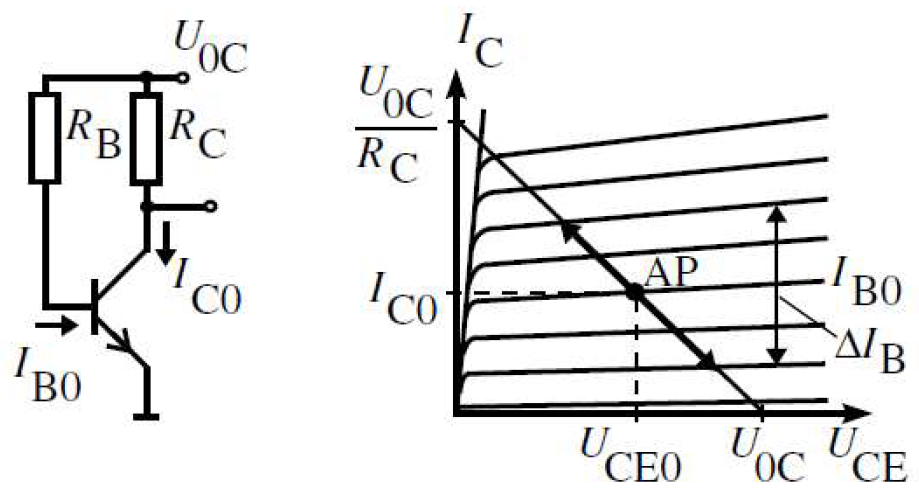
\includegraphics[width=1\textwidth]{images/emitterStufe.png}

Die Speisung VDD(U0C) sei 5V

\begin{enumerate}
\item Wie gross wird der Kollektorstrom IC0 im Arbeitspunkt, wenn die Arbeitspunkt-Spannung
UCE0=VDD/2 betragen soll?
\item Wie gross wird der Basisstrom IB0 für den Arbeitspunkt, wenn Sie einen npn-Transistor zur Verfügung haben und dieser genau den mittleren Stromverstärkungsfaktor hFE aufweist?
\item Wie gross wird die zu erwartende Basis-Emitter-Spannung VBE0 bei Ihrem Arbeitspunkt?
\end{enumerate}

\newpage
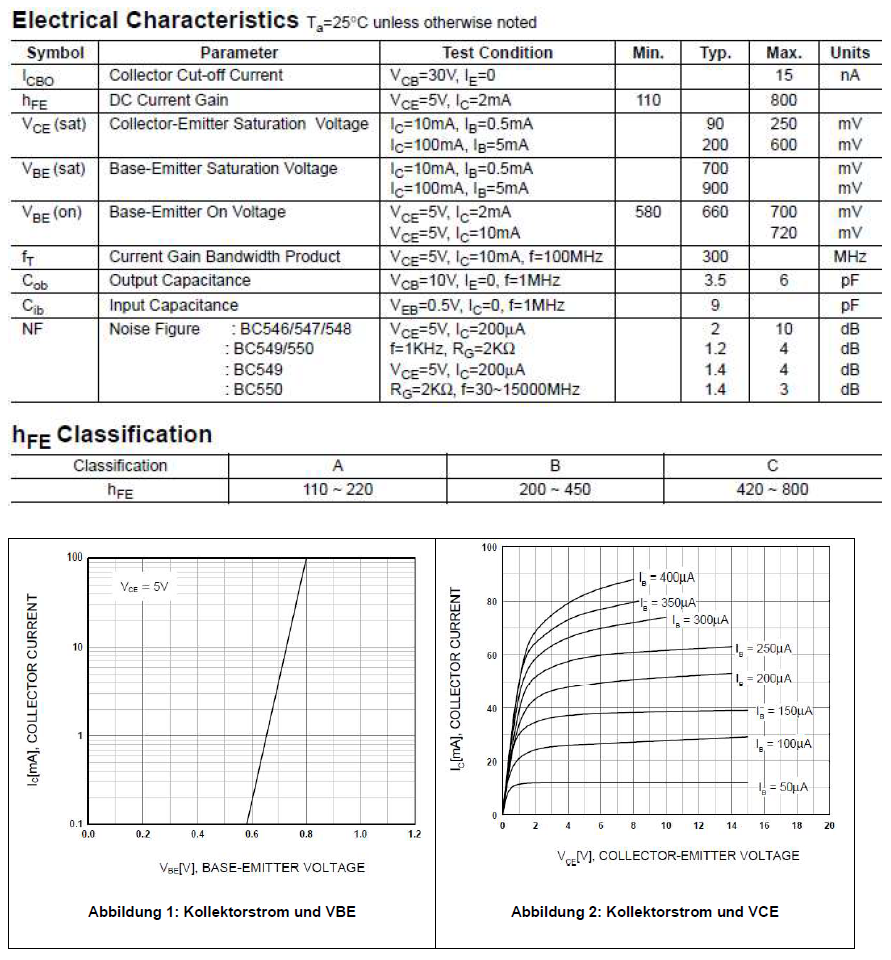
\includegraphics[width=1\textwidth]{images/datasheetBC547.png}
\newpage
\section*{Aufgabe b: Berechnung Operationsverstärkerschaltung T0454}
Gegeben ist folgende Schaltung (T0454) eines Operationsverstärkers mit geschalteten Widerständen

\includegraphics[width=1.2\textwidth]{images/opAmp.png}

Der Opamp sei ideal, d.h. er habe unendliche Verstärkung und Eingangswiderstand,keine Offsetspannung. 
Die Schalter S2, S1 und S1 sind ideal, d.h. es fliesst kein Strom, wenn sie offen sind und es fällt keine Spannung ab, wenn sie geschlossen sind.

Schalterstellung: S2, S1 und S0 geschlossen; Vin1 = 0V, Vin2 = 1V

Für unsere Anwendung soll Vout -1.75 Volt und If 1.75 mA betragen, wobei R2 = 1kOhm, R1 = 2kOhm und R0 4kOhm beträgt.

Wie gross muss Rf sein?
\newpage
\section*{Aufgabe c: Beantwortung E-Mail}
From: pirmin.meier@company.ch\\
To: peter.hasler@company.ch\\

Hallo lieber Peter,\\\\
hiermit sende ich, wie angekündigt, die von Dir so dringend benötigten Informationen. 
Bezüglich der Weiterentwicklung im Bereich der Abteilung Forschung und Entwicklung kann ich Dir folgendes mitteilen. Ich habe mit dem Bereichsleiter T\&E unserer Division gestern ein intensives Gespräch darüber geführt. Mit Sicherheit konnte er mir auch noch nicht viel bestätigen, was aber schon feststeht und sich sicher nicht mehr ändern wird, ist folgendes: Die jetzigen Forschung und Entwicklung Räumlichkeiten werden aufgegeben und ein neues, grösseres Labor am bestehenden Firmengebäude angebaut. Dieser Anbau dürfen wir aber frühestens 2022 erwarten. Die jetzigen zur Verfügung stehenden Messmittel werden zum grossen Teil ersetzt werden, wir werden neue Digital Signal Analyzer und Kathodenstrahloszilloskope mit sechs Kanälen erhalten. Die jetzigen werden, beginnend Ende 2017 etappenweise ersetzt. Genauere Informationen dazu später. Bezüglich dem personellen Ausbau von unserem Team ist momentan eine Personalsteigerung zwischen 15-25\% in Diskussion. Diese Personen werden, beginnend 2018 rekrutiert und in die Abteilung eingegliedert.
Um noch Deine Frage wegen des zu verwendenden Transistors für die Emitterstufe (Schaltung T0455) zu beantworten, ich denke ein off-the-shelf BC547 wird dazu locker reichen. \\
Was ich nun von Dir noch benötige sind folgende Informationen:
Wie gross ist der Feedback-Widerstand des Op-Amp der Schaltung T0454?
Wann genau wirst Du im Herbst deinen WK leisten, damit ich die Personalplanung anpassen kann?
Wie ist der genaue Arbeitsstand im Gerdo-Projekt?
Wie viel Zeit hast Du in etwa aufgewendet, um den Messbericht von Pavel zu korrigieren? Ich brauche diese Angabe für die zukünftige Planung.\\\\
Vielen Dank für Deine Antwort\\\\
Gruss Pirmin

Pirmin Meier\\
El. Ing. HTL\\
Abteilungsleiter F \& E\\
The Company AG\\
6300 Zug\\
Switzerland
   
\textbf{Messbericht Schaltungsteil T0453} Verstärkerschaltung 20.04.17

Der Schaltung vom Schaltungsteil T0453 wurde von mir (Pavel Datsyuk) am 20.04.17 mit Umgebungsbedingungen normal (22 Grade Celsius, 60 Prozentes relativer Luftfeuchtigkeiten) augemessen. Der Resultat der Messung ware wie erwartet positiv ausgefallen. Ich haben die Messunge exakt gleich gemacht auch noch einmal bei 
\section*{Aufgabe e: Ausfüllen Kreuzworträtsel}
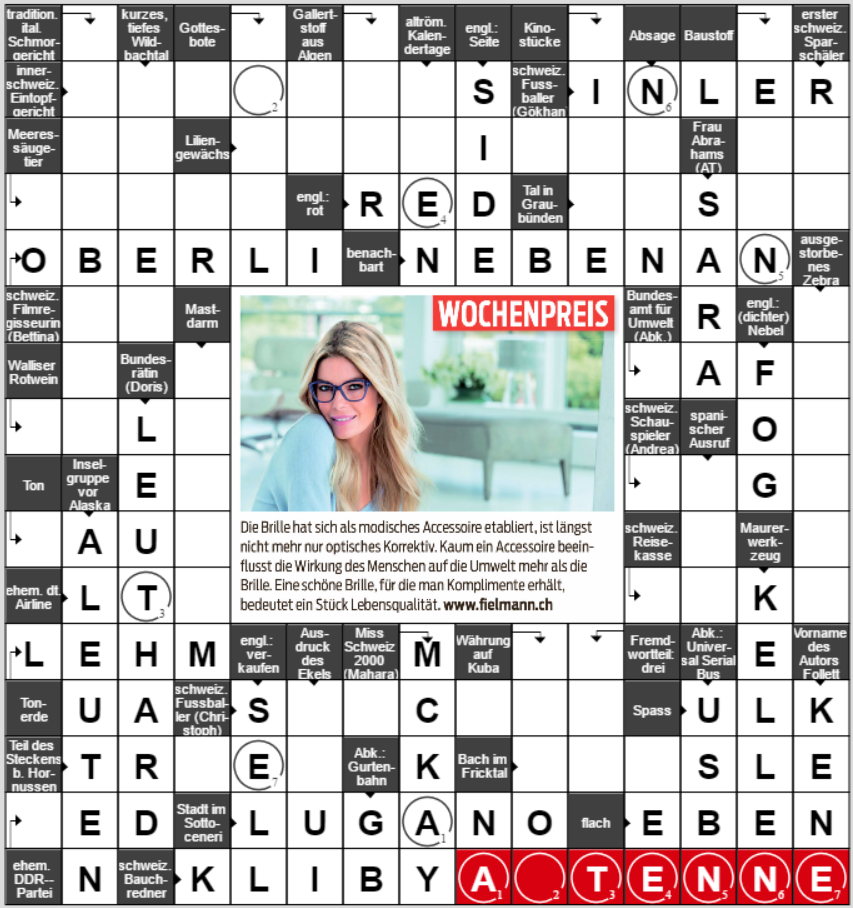
\includegraphics[width=1.2\textwidth]{images/Kreuzwortraetsel.png}
\newpage

\section*{Projektplan, Protokolle}

Datum:03.04.2017\\
Ort: HSR Rapperswil

Teilnehmer: Steve Gerome Kamga, Pascal Horat, Gökhan Kaya\\
Sitzungsleiter: Pascal Horat

Thema: Projektauftrag definieren und verstehen
\begin{enumerate}

\item Ablauf und Aufgabeplanung, Eröffnung der Sitzung 

\item  Verteilung der Aufgaben während der Sitzung
\begin{itemize}
\item Gerome: Sitzungsprotokole
\item Gökhan: Schreiben
\item Pascal: Schreiben 
\end{itemize}

\item Kontext des Projekts definieren un mögliche Fragen zum Projektsbeginn erklären.

\item Mögliche Probleme und Schwierigkeiten erwahnen

\item Regeldokument erstelen : es geht darum, allgemeiner Regeln festzulegen, welche für die Teamarbeit als verbinlich gelten.

\item Projektziele festlegen und Teamrolle gemäss Teamreview 2 beschreiben.

\item Mögliche voraussetzung für einen erfolreichen Projektmanagement definieren

\item Benötigte Literatur: HSR Projektauftrag.docx   

\item Zusammenfassung

\end{enumerate}

Nächste Sitzung: 13.04.2017




\newpage

\section*{Projektplan, Protokolle}

Datum:13.04.2017\\
Ort: HSR Rapperswil

Teilnehmer: Steve Gerome Kamga, Pascal Horat, Gökhan Kaya\\
Sitzungsleiter: keiner

Thema: Klärung der Aufgabenstellung

\begin{enumerate}

\item Ablauf und Aufgabeplanung, Eröffnung der Sitzung 

\item  Verteilung der Aufgaben während der Sitzung
\begin{itemize}
\item Gerome: Sitzungsprotokole
\item Gökhan: Interviewleitfaden erstellen
\item Pascal: MS-Projekt
\end{itemize}

\item GrobePlanung mit Microsoft Projekt erstellen: Damit jeder von uns immer immer auf das Projekt zugreifen kann.

\item Detailplanung erstellen

\item Baseline erstellen und als .pdf speichern

\item Interviewleitfaden erstellen: vorhandener Fragekatalog mit Fragekatalog von Dozent erweitern, Raster für Koordinaten des Befragten erstellen, Frage hinzufügen ob Befragter genannt werden will.

\item Latex-Vorlage Projektbericht organisieren

\item Benötigte Literatur: 

\item Zusammenfassung

\end{enumerate}

Nächste Sitzung: 19.04.2017

\newpage
\section*{Projektplan, Protokolle}

Datum:19.04.2017\\
Ort: HSR Rapperswil

Teilnehmer: Steve Gerome Kamga, Pascal Horat, Gökhan Kaya\\
Sitzungsleiter: keiner

Thema: Plannung un Vorgehen des Interviews (1)

\begin{enumerate}

\item Ablauf und Aufgabeplanung, Eröffnung der Sitzung 

\item  Verteilung der Aufgaben während der Sitzung
\begin{itemize}
\item Gerome: Sitzungsprotokole
\item Gökhan: 
\item Pascal: 
\end{itemize}

\item	Projektbericht Template erstellen

\item  interviewleitfaden herstellen:  Mit Hilfe internets zehn Schlüsselkompetenzen auswählen.

\item 	interviewPartner für Beschaffung der Kernkompetenzen notieren: Jeder notiert sich 3 mögliche Partner, die er kontaktieren könnte. damit wir   sicherstellen können, dass jeder am Schluss Kontakt mit ca. 2 Partnern hatte.

\item 	Terminvorschlag mit mögliche Interviewpartner festlegen:  Die Termine sind in unserem Auftragsdokument in Excel unter Tab «Projektpartner» zu notieren.

\item	Antwortformulare Einfordern : Formulare mit Namen der befragten Person beschriften und unter OneDrive/TKI /ProjektAC/Befragung abspeichern.


\item Latex-Vorlage Projektbericht organisieren

\item Benötigte Literatur: Simon 2002   \cite{simon2002entwicklung}

\item Zusammenfassung

\end{enumerate}

Nächste Sitzung: 05.05.2017

\newpage
\section*{Projektplan, Protokolle}

Datum:05.05.2017\\
Ort: HSR Rapperswil

Teilnehmer: Steve Gerome Kamga, Pascal Horat, Gökhan Kaya\\
Sitzungsleiter: keiner

Thema: Auswertung der Interview

\begin{enumerate}

\item Ablauf und Aufgabeplanung, Eröffnung der Sitzung 

\item  Verteilung der Aufgaben während der Sitzung
\begin{itemize}
\item Gerome: Sitzungsprotokole
\item Gökhan: 
\item Pascal: 
\end{itemize}

\item	Projekt anpassen gemäss plan.


\item 	Übersichtsdokument der Kompetenzen erstellen :In diesem Dokument sollten alle Antworten der Formulare eingetragen und dann ausgewertet werden. Dieses Dokument wird optimalerweise direkt in Projektbericht verfasst.

\item 	Kernkompetenzen ermitteln.

\item 	An Projektbericht weiter schreiben

\item Benötigte Literatur: Simon 2002   \cite{simon2002entwicklung}

\item Zusammenfassung

\end{enumerate}

Nächste Sitzung: 14.05.2017

\newpage
\section*{Projektplan, Protokolle}

Datum:14.05.2017\\
Ort: HSR Rapperswil

Teilnehmer: Steve Gerome Kamga, Pascal Horat, Gökhan Kaya\\
Sitzungsleiter: keiner

Thema: überlegung über Beobachtungsinstrument
\begin{enumerate}

\item Ablauf und Aufgabeplanung, Eröffnung der Sitzung 

\item  Verteilung der Aufgaben während der Sitzung
\begin{itemize}
\item Gerome: Sitzungsprotokole
\item Gökhan: 
\item Pascal: 
\end{itemize}


\item  Die wichtigsten Kernkompetenzen selektieren:
\begin{itemize}
\item Analytisches und systematisches Denken
\item Lernbereitschaft und Lernfähigkeit
\item Selbstmanagement und Selbstorganisation 
\end{itemize}

\item mögliche Ideen zum Beobachtungsinstrument vorschlagen: es geht darum zwei übungen zu entwickeln,  mit denen sich die fünf von uns gewählten Kernkompetenzen herauskristalisiernen lassen

\item Erzeugung Von Übungen zum Testen der Kernkompetenzen

\item Powerpoint Vorlage für die Präsentation vorbereiten	

\item Probanten für den Test der Kernkompetenzen auswählen


\item Benötigte Literatur: 

\item Zusammenfassung

\end{enumerate}

Nächste Sitzung: 19.05.2017

\newpage
\section*{Projektplan, Protokolle}

Datum:19.05.2017\\

Ort: HSR Rapperswil

Teilnehmer: Steve Gerome Kamga, Gökhan Kaya\\

Sitzungsleiter: keiner

Thema: Erstellung der Projektpräsentation
\begin{enumerate}

\item Ablauf und Aufgabeplanung, Eröffnung der Sitzung 

\item  Verteilung der Aufgaben während der Sitzung
\begin{itemize}
\item Gerome: 
\item Gökhan: 
\end{itemize}

\item PowerPoint erzeugen und einrichten

\item Präsentation üben


\item Benötigte Literatur: 

\item Zusammenfassung

\end{enumerate}

Nächste Sitzung: 01.06.2017



\newpage
\section*{Projektplan, Protokolle}

Datum:01.06.2017\\
Ort: HSR Rapperswil

Teilnehmer: Steve Gerome Kamga, Pascal Horat, Gökhan Kaya\\
Sitzungsleiter: keiner

Thema: Bewertung der Probanten
\begin{enumerate}

\item Ablauf und Aufgabeplanung, Eröffnung der Sitzung 

\item  Verteilung der Aufgaben während der Sitzung
\begin{itemize}
\item Gerome: Sitzungsprotokole
\item Gökhan: 
\item Pascal: 
\end{itemize}



\item Resultate der einzelnen Probanten analysieren, interpretieren und schön darstellen 		

\item 	Projektauftrag weiter schreiben

\item 	Bewertung der Ergebnissen von Beobachtungsinstrument


\item Benötigte Literatur

\item Zusammenfassung

\end{enumerate}

Nächste Sitzung: 07.06.2017

\newpage
\section*{Projektplan, Protokolle}

Datum:07.06.2017\\
Ort: HSR Rapperswil

Teilnehmer: Steve Gerome Kamga, Pascal Horat, Gökhan Kaya\\
Sitzungsleiter: keiner

Thema: Projektbericht fertigstellen
\begin{enumerate}

\item Ablauf und Aufgabeplanung, Eröffnung der Sitzung 

\item  Verteilung der Aufgaben während der Sitzung
\begin{itemize}
\item Gerome: Sitzungsprotokole
\item Gökhan: Auswertung der Übungen schreiben
\item Pascal: Bericht erweitern
\end{itemize}

\item Bewertungsergebnisse zur Lernbereitschaft und Lernfähigkeit

\item Verfassung der Übungsauswertung, Kapitel 3 (Klärung Projektauftrag)  sowie Zusammenfassung im Projektbericht 

\item Auswertung Assesment in Projektbericht

\item Interview ausbauen und Reflexion Verfassen

\item Schlussfolgerungen, Ausblicke und Empfehlungen verfassen 

\item Zusammenfassung

\end{enumerate}

Nächste Sitzung: 8.06.2017

\newpage

\section*{Übersichtausschnitt der Auftragsaufteilung}

%\begin{tabular}{ | l | l | l |}
 %\begin{tabular}{ | p{7cm} | p{4cm} | p{2cm} |}
 \begin{longtable}{ | p{7cm} | p{4cm} | p{2cm} |}
   \hline
   \textbf{Auftrag} & \textbf{Verfasser} & \textbf{Zeit[min]}   \\
   \hline  		
    Microsoft Project einrichten & Gerome & 60 \\ \hline
    Detailplanung erstellen & Pascal & 180 \\ \hline
    Baseline erstellen  & Pascal & 30 \\ \hline
    Interviewleitfaden erstellen& Gökhan,Gerome & 180 \\ \hline
    LaTeX-Vorlage Projektbericht organisieren & Pascal, Gökhan & 100 \\ \hline
    Lernbilanz 2 & Pascal, Gerome,Gökhan & \\ \hline
    lernbilanz 3 & Pasacl, Gerome,Gökhan &  \\ \hline
    Projektbericht Template erstellen & Gökhan & 120 \\ \hline
    Partner für Beschaff. Kernkomp. notieren & Pascal,Gerome,Gökhan & 30 \\ \hline
    Projektplan anpassen gemäss Angaben & Pascal & 120 \\ \hline
    Termine Interviewpartner festlegen & Pascal, Gerome, Gökhan & 30 \\ \hline
    Formulare versenden & Pascal, Gerome Göhkan & 15 \\ \hline
    Antwortformulare Einfordern & Pascal, Gerome, Gökhan & 10 \\ \hline
    Übersichtsdok. Kompetenzen erstellen & Gökhan & 60 \\ \hline    
    Kernkompetenzen ermitteln & Gerome,Gökhan & 10 \\ \hline   
    an Projektbericht schreiben & Gökhan & 90 \\ \hline   
    Punkt c im File AuftragAC\_ersteLektion.png erledigen &  &  \\ \hline    
    Aufgabe entwickeln oder finden um die Kernkompetenz Lernbereitschaft zu testen  & Pascal &  \\ \hline   
    Aufgabe entwickeln oder finden um die Kernkompetenz Selbstmanagement zu testen  & Gökhan & 90 \\ \hline  
    Teamsitzungsprotokolle erstellen & Gerome & 100 \\ \hline    
    Analyse Projektauftrag in main.tex einbringen, Vorlage in HSR\_Projektauftrag.docx & Gerome, Gökhan & 20\\ \hline   
    Übersicht erstellen wer wie viel Zeit für was investiert hat im Projekt TKI & Gerome & 60\\ \hline   
    Commit-History in 06vorgehen.tex schön formatieren & Gerome & 30 \\ \hline 
    Auswertung der Übung in Projektbericht verfassen  & Pascal, Gökhan & 480 \\ \hline   
Auswertung des Assessments in Projektbericht verfassen & Pascal, Gökhan & 200 \\ \hline  
Zusammenfassung auf Seite 2 in Projektbericht verfassen     & Pascal &  \\ \hline   
Commit-History aus Git extrahieren und in Latex erweitern, in Anhang von Projektbericht verschieben     & Gerome & 30 \\ \hline
 Verzeichnisse (Kapitel 1) einfügen in Projektbericht    &  &  \\ \hline  
 Einleitung erweitern    & Pascal &  \\ \hline   
 Kapitel 3 verfassen (Klärung Projektauftrag)    & Pascal &  \\ \hline
 Formattierung Projektbericht verbessern (inkl. Unterschriften in Kapitel 4)    & Pascal, Gökhan &  \\ \hline  
 Kapitel 7 Interview ausbauen  & Pascal, Gökhan &  \\ \hline   
 Kapitel 11 Reflexion verfassen & Pascal, Gökhan &  \\ \hline    
 Kapitel 12 Schlussfolgerungen, Ausblicke und Empfehlungen    verfassen & Pascal, Gökhan &  \\ \hline  
 Erklärung Urheberschaft einfügen & Pascal & 30 \\ \hline   
 Anhang in Projektbericht erweitern & Gerome &  \\ \hline     
 Tabelle Übersichtausschnitt der Auftragsaufteilung in Projektbericht aktualisieren anhand \_Aufträge.xlsx    & Gerome &  \\ \hline    
     &  &  \\ \hline  
     
%\end{tabular}
\end{longtable}
     
\newpage

\section*{Commit History}
 


%AB HIER KANN JEROME FORMATIEREN
SteveGerome, Thu Jun 8 14:41:41 2017 +0200 : übersichtausschnitt Auftragsaufteilung 2 \\
SteveGerome, Thu Jun 8 13:38:13 2017 +0200 : übersichtausschnitt Auftragsaufteilung 1 \\
SteveGerome, Thu Jun 8 08:27:47 2017 +0200 : übersichtausschnitt Auftragsaufteilung \\
kaya, Wed Jun 7 15:45:05 2017 +0200 : Bewertung fertiggestellt. Noch kommentieren \\
Corumh, Wed Jun 7 14:35:31 2017 +0200 : Alles zusammen kompiliert \\
kaya, Wed Jun 7 14:28:50 2017 +0200 : Merge branch 'master' of https://github.com/cruis1/tki Konflikt \\
kaya, Wed Jun 7 14:28:35 2017 +0200 : Ein Teil der Bewertung geschrieben \\
Corumh, Wed Jun 7 14:24:53 2017 +0200 : Auswertung Assessment weitergeschrieben \\
Corumh, Wed Jun 7 12:00:57 2017 +0200 : Auswertung der Übung 2 weitergeschr. \\
Corumh, Wed Jun 7 11:08:15 2017 +0200 : Auswertung des Assessments weitergeschr. \\
Corumh, Wed Jun 7 10:49:07 2017 +0200 : Auswertung des Assessments angefangen \\
Corumh, Wed Jun 7 09:37:18 2017 +0200 : Bewertungsanmerkungen Probanden angefangen \\
Corumh, Wed Jun 7 09:15:48 2017 +0200 : Bewertungstabellen Probanden fertig \\
Corumh, Tue Jun 6 19:47:35 2017 +0200 : Protokolle angepasst \\
SteveGerome, Tue Jun 6 19:38:49 2017 +0200 : Sitzungsprotokolle verbessert 1 \\
SteveGerome, Tue Jun 6 19:32:49 2017 +0200 : Sitzungsprotokolle verbesssert \\
SteveGerome, Tue Jun 6 15:20:25 2017 +0200 : Commit History form. beendet \\
Corumh, Tue Jun 6 15:06:20 2017 +0200 : Bewertung Probanden Selbstmanagement gem. \\
Corumh, Tue Jun 6 13:28:31 2017 +0200 : Bewertung Probanden weitergeschr. \\
Corumh, Tue Jun 6 13:05:02 2017 +0200 : Bewertung Probanden angefangen \\
Corumh, Tue Jun 6 12:25:31 2017 +0200 : Einleitung angepasst \\
Corumh, Tue Jun 6 12:20:58 2017 +0200 : gitignore angepasst \\
Corumh, Tue Jun 6 12:16:57 2017 +0200 : gitignore angepasst \\
Corumh, Tue Jun 6 12:14:32 2017 +0200 : gitignore angepasst \\
Corumh, Tue Jun 6 11:58:05 2017 +0200 : Ablauf Assessment beschr. \\
SteveGerome, Tue Jun 6 11:54:51 2017 +0200 : Commit History form. beendet \\
SteveGerome, Tue Jun 6 11:34:53 2017 +0200 : Commit History form. weiter verbe. \\
kaya, Tue Jun 6 11:25:39 2017 +0200 : Merge branch 'master' of https://github.com/cruis1/tki Merge \\
kaya, Tue Jun 6 11:25:24 2017 +0200 : Mainfile Projektauftrag hinzugefügt \\
Corumh, Tue Jun 6 11:22:24 2017 +0200 : Merge branch 'master' of https://github.com/cruis1/tki \\
Corumh, Tue Jun 6 11:21:39 2017 +0200 : Commit History Formattierung verb. \\
kaya, Tue Jun 6 11:21:37 2017 +0200 : Filevorlage Projektauftrag erstellt \\
SteveGerome, Tue Jun 6 11:15:50 2017 +0200 : Commit History form. verb. \\
SteveGerome, Tue Jun 6 11:09:43 2017 +0200 : trying \\
SteveGerome, Tue Jun 6 11:08:57 2017 +0200 : trying \\
SteveGerome, Tue Jun 6 11:05:35 2017 +0200 : trying \\
SteveGerome, Tue Jun 6 11:02:12 2017 +0200 : trying \\
Corumh, Tue Jun 6 10:54:42 2017 +0200 : gitignore Assessment erstellt \\
kaya, Tue Jun 6 10:30:00 2017 +0200 : Commit history hinzugefügt \\
kaya, Thu Jun 1 16:15:20 2017 +0200 : Diverse Änderungen im Abschnit Teamgrundlagen und Vorgehen \\
kaya, Thu Jun 1 15:32:12 2017 +0200 : Merge branch 'master' of https://github.com \\
kaya, Thu Jun 1 16:15:20 2017 +0200 : Diverse Änderungen im Abschnitt Teamgrundlagen und Vorgehen \\
kaya, Thu Jun 1 15:32:12 2017 +0200 : Merge branch 'master' of https://github.com/cruis1/tki merge \\
kaya, Thu Jun 1 15:32:03 2017 +0200 : Teil Vorgehen überarbeitet \\
Corumh, Thu Jun 1 15:25:52 2017 +0200 : Übung Selbstmanag. mitzut. Infos fertigg. \\
kaya, Thu Jun 1 14:44:34 2017 +0200 : Merge branch 'master' of https://github.com/cruis1/tki böö \\
kaya, Thu Jun 1 14:44:23 2017 +0200 : Teil Vorgehen geschrieben \\
Corumh, Thu Jun 1 14:42:44 2017 +0200 : Übung Selbstmanag. mitzut. Infos angef. \\
Corumh, Thu Jun 1 13:58:12 2017 +0200 : Übung Selbstmanag. verfeinert \\
Corumh, Thu Jun 1 13:19:40 2017 +0200 : Merge branch 'master' of https://github.com/cruis1/tki \\
Corumh, Wed May 31 17:51:22 2017 +0200 : Übung Selbstmanag. alle Aufgabe fertig \\
kaya, Wed May 31 16:02:27 2017 +0200 : Teil Klärung der Aufgabenstellung angefangen \\
kaya, Wed May 31 15:31:15 2017 +0200 : Merge branch 'master' of https://github.com/cruis1/tki kei ahnig was lauft \\
kaya, Wed May 31 15:28:27 2017 +0200 : Fragetext korrigiert \\
Corumh, Wed May 31 15:22:57 2017 +0200 : Merge branch 'master' of https://github.com/cruis1/tki \\
Corumh, Wed May 31 15:22:32 2017 +0200 : Übung Selbstmanag. E-Mail-Aufgabe fertig \\
kaya, Wed May 31 15:12:52 2017 +0200 : Einleitung korrigiert \\
kaya, Wed May 31 14:46:12 2017 +0200 : Kapitel Teamgrundlagen geschrieben. Achtung: Kann fehler verursachen beim kompilieren \\
kaya, Wed May 31 12:17:54 2017 +0200 : Vorbereitungen für Teamvertrag img ordner hinzugefügt \\
Corumh, Wed May 31 12:16:43 2017 +0200 : Übung Selbstmanag. Kreuzwortraetsel fertig \\
kaya, Wed May 31 11:51:52 2017 +0200 : Erster Teil der Einleitung \\
Corumh, Wed May 31 11:48:57 2017 +0200 : Übung Selbstmanag. Messbericht fast fertig \\
kaya, Wed May 31 10:56:55 2017 +0200 : kleine korrekturen \\
Corumh, Wed May 31 10:49:15 2017 +0200 : Übung Selbstmanag. Messbericht weitergeschr. \\
kaya, Wed May 31 10:40:43 2017 +0200 : Merge branch 'master' of https://github.com/cruis1/tki testmerge \\
kaya, Wed May 31 10:40:15 2017 +0200 : Tabelle korrigiert \\
Corumh, Wed May 31 10:39:52 2017 +0200 : Übung Selbstmanag. Messbericht angef. \\
Kaya, Tue May 30 20:30:33 2017 +0200 : Diverse Tabellen hinzugefügt \\
Kaya, Tue May 30 19:56:43 2017 +0200 : Viele Korrekturen und weitere Arbeiten \\
kaya, Tue May 30 18:11:52 2017 +0200 : Teil Test1 hinzugefügt \\
Corumh, Tue May 30 16:27:24 2017 +0200 : Übung Selbstmanag. Bewertungskriterien weiter beschr. \\
Corumh, Tue May 30 15:19:04 2017 +0200 : Beobachtungsinstr. Selbstmanag. Bewertungskriterien beschr. \\
kaya, Tue May 30 14:47:56 2017 +0200 : nüt \\
Corumh, Tue May 30 14:29:34 2017 +0200 : Beobachtungsinstr. Selbstmanag. Bewertung \\
Corumh, Tue May 30 13:53:05 2017 +0200 : Beobachtungsinstr. Selbstmanag. Aufgaben weiter beschrieben \\
Corumh, Mon May 29 17:14:46 2017 +0200 : Beobachtungsinstr. Selbstmanag. Aufgaben beschrieben \\
Corumh, Mon May 29 16:10:04 2017 +0200 : Beobachtungsinstr. Selbstmanag. Detail beschrieben \\
Corumh, Mon May 29 16:06:30 2017 +0200 : Beobachtungsinstr. Selbstmanag. weiter beschrieben \\
Corumh, Mon May 29 15:56:12 2017 +0200 : Beobachtungsinstr. Selbstmanag. beschrieben \\
Kaya, Thu May 25 20:42:47 2017 +0200 : Korrekturen und weitere Arbeiten \\
Corumh, Sun May 14 16:07:20 2017 +0200 : Projektbericht Fehler behoben \\
kaya, Mon May 8 16:01:52 2017 +0200 : readme update \\
kaya, Mon May 8 16:00:37 2017 +0200 : readme update \\
kaya, Mon May 8 15:52:42 2017 +0200 : korrekturen \\
kaya, Mon May 8 15:40:18 2017 +0200 : Kernkompetenz Auswertung hinzugefügt, Assessmentbericht Interviewteil weitergeschrieben \\
kaya, Mon May 8 14:59:29 2017 +0200 : HILFE file überarbeitet \\
kaya, Mon May 8 14:58:12 2017 +0200 : HILFE file erstellt für die hartnäckige merge konflikt \\
Corumh, Mon Apr 24 16:35:48 2017 +0200 : Projektbericht Referenz Website \\
kaya, Mon Apr 24 16:31:32 2017 +0200 : ksjdksj \\
Corumh, Mon Apr 24 16:26:53 2017 +0200 : Projektbericht Referenz Website \\
Corumh, Mon Apr 24 16:26:05 2017 +0200 : Projektbericht Referenz Website \\
kaya, Mon Apr 24 16:21:51 2017 +0200 : nüt spannends \\
kaya, Mon Apr 24 15:11:00 2017 +0200 : Ordner Projektbericht gelöscht \\
kaya, Mon Apr 24 12:12:08 2017 +0200 : Fragekatalog verbessert 2 \\
kaya, Mon Apr 24 12:05:55 2017 +0200 : Fragenkatalog korrigiert \\
kaya, Wed Apr 19 19:09:19 2017 +0200 : Assessmentbericht template fertig \\
kaya, Wed Apr 19 15:34:54 2017 +0200 : Fragekatalog nachgebessert \\
kaya, Wed Apr 12 21:02:19 2017 +0200 : Fragenkatalog angepasst \\
Corumh, Mon Apr 3 23:26:16 2017 +0200 : TR3 Orthografie korrigiert \\
Corumh, Mon Apr 3 23:02:35 2017 +0200 : TR3 komplett überarbeitet \\
Corumh, Mon Apr 3 20:29:41 2017 +0200 : TR3 Protokoll eingefügt \\
kaya, Mon Apr 3 20:00:33 2017 +0200 : TR3 fast fertig \\
kaya, Mon Apr 3 18:45:59 2017 +0200 : Gruppeneinschätzung fertig \\
kaya, Mon Apr 3 16:48:33 2017 +0200 : TR3 continue \\
Corumh, Mon Apr 3 16:01:09 2017 +0200 : TR3 Web-Pic eingefügt \\
Corumh, Mon Apr 3 15:57:15 2017 +0200 : Merge branch 'master' of https://github.com/cruis1/tki \\
kaya, Mon Apr 3 15:56:59 2017 +0200 : Arbeit... \\
Corumh, Mon Apr 3 14:52:12 2017 +0200 : TR2 Änderig\\
Corumh, Mon Apr 3 14:08:39 2017 +0200 : TR3 Vorlage pagebreak entfernt\\
kaya, Mon Apr 3 14:04:13 2017 +0200 : TR3 vorlage angepasst\\
Corumh, Mon Apr 3 02:27:49 2017 +0200 : TR3 Vorlage Fehler entfernt\\
kaya, Mon Mar 27 16:41:16 2017 +0200 : nichts nennenswertes\\
Corumh, Mon Mar 27 15:50:50 2017 +0200 : TR3 Vorlage angefangen\\
Corumh, Mon Mar 27 12:11:55 2017 +0200 : TR2 in finale Form gebracht\\
kaya, Mon Mar 27 11:08:49 2017 +0200 : pagebreak aenderungen auskommentiert\\
Corumh, Mon Mar 27 01:59:09 2017 +0200 : TR2 zusätzliche Literatur eingefügt\\
Corumh, Mon Mar 27 00:38:32 2017 +0200 : TR2 kompl. überarb. (Rechtschreibef.) und erweitert\\
Corumh, Sun Mar 26 17:45:31 2017 +0200 : TR2 fast fertig\\
Corumh, Sun Mar 26 15:27:03 2017 +0200 : an TR2 weitergearbeitet\\
SteveGerome, Sun Mar 26 15:16:44 2017 +0200 : weitergeschrieben TR2\\
Corumh, Sun Mar 26 14:55:44 2017 +0200 : an TR2 weitergearbeitet, Bilder eingefügt\\
Corumh, Thu Mar 23 14:24:16 2017 +0100 : an TR2 weitergearbeitet, Bilder eingefügt\\
Corumh, Thu Mar 23 14:03:00 2017 +0100 : .rtf gelöscht\\
Corumh, Thu Mar 23 13:59:07 2017 +0100 : .log gelöscht\\
Corumh, Thu Mar 23 13:57:40 2017 +0100 : TR2 Formattierung verschönert und weitergeschrieben\\
Corumh, Thu Mar 23 13:16:42 2017 +0100 : TR2 weitergearbeitet\\
SteveGerome, Wed Mar 22 21:23:31 2017 +0100 : zweiter Commit :-)\\
Corumh, Wed Mar 22 21:18:40 2017 +0100 : einige Korrekturen in TR2\\
SteveGerome, Wed Mar 22 21:15:22 2017 +0100 : erster Commit :-)\\
Corumh, Wed Mar 22 20:27:56 2017 +0100 : neueste Teamreview 2 Version Upload\\
kaya, Wed Mar 22 20:22:35 2017 +0100 : shit happened\\
kaya, Wed Mar 22 20:15:19 2017 +0100 : Selbsteinschätzung bearbeitet\\
Corumh, Wed Mar 22 20:10:43 2017 +0100 : hoffentlich klappts\\
kaya, Wed Mar 22 20:06:50 2017 +0100 : Merge branch 'master' of https://github.com/cruis1/tki\\
kaya, Wed Mar 22 20:06:26 2017 +0100 : Selbsteinschätzung überarbeitet\\
Corumh, Wed Mar 22 20:05:09 2017 +0100 : hoffentlich klappts\\
kaya, Wed Mar 22 19:45:55 2017 +0100 : Merge branch 'master' of https://github.com/cruis1/tki\\
kaya, Wed Mar 22 19:44:30 2017 +0100 : Fremdeinschätzung grob ferig\\
Corumh, Wed Mar 22 19:34:07 2017 +0100 : zum Abgliche\\
Corumh, Wed Mar 22 19:02:33 2017 +0100 : resolve merge error\\
Corumh, Wed Mar 22 18:45:58 2017 +0100 : Teamreview 2 Selbsteinsch. bearb\\
kaya, Wed Mar 22 18:45:31 2017 +0100 : test\\
kaya, Wed Mar 22 18:38:25 2017 +0100 : Merge branch 'master' of https://github.com/cruis1/tki\\
kaya, Wed Mar 22 18:34:32 2017 +0100 : removed Fremdeinschätzung\\
Corumh, Wed Mar 22 18:32:15 2017 +0100 : Teamreview 2 Selbsteinsch. bearb\\
kaya, Wed Mar 22 18:23:28 2017 +0100 : selbsteinschätzung erstellt\\
kaya, Wed Mar 22 17:04:09 2017 +0100 : selbsteinschätzung erstellt\\
Corumh, Tue Mar 21 17:35:53 2017 +0100 : Teamreview 2 weitererstellt, Referenzen funktionieren\\
Corumh, Tue Mar 21 17:32:52 2017 +0100 : Teamreview 2 weitererstellt, Referenzen funktionieren\\
Corumh, Tue Mar 21 13:56:24 2017 +0100 : Teamreview 2 Struktur erstellt, Referenzen funktionieren\\
Corumh, Tue Mar 21 12:09:38 2017 +0100 : Teamreview 2 Template angefangen\\
Corumh, Tue Mar 21 11:30:41 2017 +0100 : Ordnerstruktur geändert und noch mehr aufgeräumt\\
Corumh, Tue Mar 21 11:18:35 2017 +0100 : Ordnerstruktur geändert und aufgeräumt\\
Corumh, Tue Mar 21 11:10:12 2017 +0100 : Upload TR2\\
Corumh, Mon Mar 20 20:12:37 2017 +0100 : Penis\\
Corumh, Mon Mar 20 19:28:05 2017 +0100 : Upload TR2\\
Corumh, Mon Mar 20 16:13:56 2017 +0100 : Upload TR2\\
Corumh, Mon Mar 20 15:07:02 2017 +0100 : Upload TR2\\
Corumh, Mon Mar 20 13:58:25 2017 +0100 : Upload Vorlage TR2\\
Corumh, Mon Mar 20 12:29:35 2017 +0100 : Reflexion Sitzung finalisiert\\
Corumh, Fri Mar 17 17:07:49 2017 +0100 : Reflexion Sitzung erstellt\\
Corumh, Fri Mar 17 16:22:08 2017 +0100 : Traktl. final.\\
Corumh, Thu Mar 16 20:41:02 2017 +0100 : Upload Traktl. akt.\\
Corumh, Thu Mar 16 20:10:54 2017 +0100 : Upload Traktl.\\
Corumh, Thu Mar 16 19:40:46 2017 +0100 : Konflikt bereinige\\
Corumh, Mon Mar 13 20:53:49 2017 +0100 : Reflexion TR1 erstellt\\
kaya, Mon Mar 13 17:19:59 2017 +0100 : Merge branch 'master' of https://github.com/cruis1/tki\\
kaya, Mon Mar 13 17:06:10 2017 +0100 : Name angepasst\\
kaya, Mon Mar 13 17:04:04 2017 +0100 : Name angepasst\\
kaya, Mon Mar 13 17:02:42 2017 +0100 : Name angepasst\\
Corumh, Mon Mar 13 16:46:47 2017 +0100 : Reflexion TR1 erstellt\\
kaya, Mon Mar 13 16:32:36 2017 +0100 : Änderungen an trakdandenliste\\
kaya, Mon Mar 13 16:13:56 2017 +0100 : Trakdandenliste explizit vervollständigt\\
kaya, Mon Mar 13 15:42:03 2017 +0100 : Fragenkatalog fertiggestellt\\
kaya, Mon Mar 13 15:10:35 2017 +0100 : Fragenkatalog Vorlage erstellt\\
kaya, Mon Mar 13 14:31:25 2017 +0100 : Fragenkatalog erstellt\\
Corumh, Mon Mar 13 12:35:32 2017 +0100 : Merge branch 'master' of https://github.com/cruis1/tki\\
Corumh, Mon Mar 13 12:34:18 2017 +0100 : Regeldokument finalisiert\\
Columh, Sun Mar 12 23:49:13 2017 +0100 : Add files via upload\\
kaya, Sun Mar 12 20:20:00 2017 +0100 : trakdandenliste\_vorlage grob fertig\\
kaya, Sun Mar 12 18:50:06 2017 +0100 : trakdandenliste erstellt\\
Corumh, Thu Mar 9 17:49:18 2017 +0100 : Regeldokument erweitert mit Bildern\\
Corumh, Thu Mar 9 10:47:33 2017 +0100 : Regeldokument erweitert\\
Corumh, Tue Mar 7 13:54:55 2017 +0100 : Regeldokument erstellt\\
kaya, Mon Mar 6 16:56:25 2017 +0100 : Aufträge aktualisiert\\
kaya, Mon Mar 6 16:29:39 2017 +0100 : teamreview update\\
kaya, Mon Mar 6 15:29:30 2017 +0100 : teamreview bearbeitet\\
kaya, Mon Mar 6 14:55:55 2017 +0100 : Ordner umbenannt und teamreview erstellt\\
Corumh, Mon Mar 6 14:07:14 2017 +0100 : LaTex Template verbessert\\
Corumh, Mon Mar 6 14:01:18 2017 +0100 : LaTex Template erstellt\\
Corumh, Mon Mar 6 12:02:56 2017 +0100 : LaTex Template angefangen\\
Corumh, Sun Mar 5 20:23:42 2017 +0100 : ToDo angepasst\\
cruis1, Sun Mar 5 00:18:42 2017 +0100 : Delete\_config.yml\\
kaya, Sun Mar 5 00:14:02 2017 +0100 : Merge branch 'master' of https://github.com/cruis1/tki\\
cruis1, Sun Mar 5 00:10:44 2017 +0100 : Delete\_config.yml\\
kaya, Sun Mar 5 00:04:13 2017 +0100 : doodle zu moodle geändert :)\\
cruis1, Sun Mar 5 00:01:11 2017 +0100 : Set theme jekyll-theme-cayman\\
kaya, Sat Mar 4 23:52:00 2017 +0100 : Alle files synchronisiert md file update\\
kaya, Sat Mar 4 23:36:00 2017 +0100 : Links hinzugefügt\\
cruis1, Sat Mar 4 23:31:16 2017 +0100 : Delete new.md\\
kaya, Sat Mar 4 23:09:51 2017 +0100 : edit readme and add new.md s\\
cruis1, Sat Mar 4 22:15:50 2017 +0100 : Initial commit\\
%BIS HIER

%BEFEHL: git log --pretty=format:"%an, %ar : %s"
%BEFEHL evt. besser: git log --pretty=format:"%an, %ad : %s"
%https://git-scm.com/book/tr/v2/Git-Basics-Viewing-the-Commit-History
    
   


\end{document}
